
%%%% Generic manuscript mode, required for submission
%%%% and peer review
\documentclass[manuscript,screen,review]{acmart}
%% Fonts used in the template cannot be substituted; margin
%% adjustments are not allowed.
%%
%% \BibTeX command to typeset BibTeX logo in the docs
\AtBeginDocument{%
  \providecommand\BibTeX{{%
    \normalfont B\kern-0.5em{\scshape i\kern-0.25em b}\kern-0.8em\TeX}}}

%% Rights management information.  This information is sent to you
%% when you complete the rights form.  These commands have SAMPLE
%% values in them; it is your responsibility as an author to replace
%% the commands and values with those provided to you when you
%% complete the rights form.
\setcopyright{acmcopyright}
\copyrightyear{2018}
\acmYear{2018}
\acmDOI{10.1145/1122445.1122456}

%% These commands are for a PROCEEDINGS abstract or paper.
\acmConference[Woodstock '18]{Woodstock '18: ACM Symposium on Neural
  Gaze Detection}{June 03--05, 2018}{Woodstock, NY}
\acmBooktitle{Woodstock '18: ACM Symposium on Neural Gaze Detection,
  June 03--05, 2018, Woodstock, NY}
\acmPrice{15.00}
\acmISBN{978-1-4503-XXXX-X/18/06}


\usepackage{enumitem}
\usepackage{wrapfig}
\usepackage{multirow}

\newcommand{\toolname}{$\mathbb{C}^3$}
%%
%% Submission ID.
%% Use this when submitting an article to a sponsored event. You'll
%% receive a unique submission ID from the organizers
%% of the event, and this ID should be used as the parameter to this command.
%%\acmSubmissionID{123-A56-BU3}

%%
%% The majority of ACM publications use numbered citations and
%% references.  The command \citestyle{authoryear} switches to the
%% "author year" style.
%%
%% If you are preparing content for an event
%% sponsored by ACM SIGGRAPH, you must use the "author year" style of
%% citations and references.
%% Uncommenting
%% the next command will enable that style.
%%\citestyle{acmauthoryear}

%%
%% end of the preamble, start of the body of the document source.
\begin{document}

\graphicspath{{figures/}{pictures/}{images/}{./}} % where to search for the images
%%
%% The "title" command has an optional parameter,
%% allowing the author to define a "short title" to be used in page headers.
%\title{A Unified Framework for Multi-class Scatterplot Colorization}
\title{\toolname-palette: Co-saliency based Colorization for Comparing Multi-class Scatterplots}
%%
%% The "author" command and its associated commands are used to define
%% the authors and their affiliations.
%% Of note is the shared affiliation of the first two authors, and the
%% "authornote" and "authornotemark" commands
%% used to denote shared contribution to the research.
\author{Kecheng Lu}
\authornote{Both authors contributed equally to this research.}
\email{lukecheng0407@gmail.com}
\orcid{1234-5678-9012}
\author{G.K.M. Tobin}
\authornotemark[1]
\email{webmaster@marysville-ohio.com}
\affiliation{%
  \institution{Institute for Clarity in Documentation}
  \streetaddress{P.O. Box 1212}
  \city{Dublin}
  \state{Ohio}
  \country{USA}
  \postcode{43017-6221}
}

\author{Lars Th{\o}rv{\"a}ld}
\affiliation{%
  \institution{The Th{\o}rv{\"a}ld Group}
  \streetaddress{1 Th{\o}rv{\"a}ld Circle}
  \city{Hekla}
  \country{Iceland}}
\email{larst@affiliation.org}

\author{Valerie B\'eranger}
\affiliation{%
  \institution{Inria Paris-Rocquencourt}
  \city{Rocquencourt}
  \country{France}
}

\author{Aparna Patel}
\affiliation{%
 \institution{Rajiv Gandhi University}
 \streetaddress{Rono-Hills}
 \city{Doimukh}
 \state{Arunachal Pradesh}
 \country{India}}

\author{Huifen Chan}
\affiliation{%
  \institution{Tsinghua University}
  \streetaddress{30 Shuangqing Rd}
  \city{Haidian Qu}
  \state{Beijing Shi}
  \country{China}}

\author{Charles Palmer}
\affiliation{%
  \institution{Palmer Research Laboratories}
  \streetaddress{8600 Datapoint Drive}
  \city{San Antonio}
  \state{Texas}
  \country{USA}
  \postcode{78229}}
\email{cpalmer@prl.com}

\author{John Smith}
\affiliation{%
  \institution{The Th{\o}rv{\"a}ld Group}
  \streetaddress{1 Th{\o}rv{\"a}ld Circle}
  \city{Hekla}
  \country{Iceland}}
\email{jsmith@affiliation.org}

\author{Julius P. Kumquat}
\affiliation{%
  \institution{The Kumquat Consortium}
  \city{New York}
  \country{USA}}
\email{jpkumquat@consortium.net}

%%
%% By default, the full list of authors will be used in the page
%% headers. Often, this list is too long, and will overlap
%% other information printed in the page headers. This command allows
%% the author to define a more concise list
%% of authors' names for this purpose.
\renewcommand{\shortauthors}{Trovato and Tobin, et al.}

%%
%% The abstract is a short summary of the work to be presented in the
%% article.
\begin{abstract}
  A clear and well-documented \LaTeX\ document is presented as an
  article formatted for publication by ACM in a conference proceedings
  or journal publication. Based on the ``acmart'' document class, this
  article presents and explains many of the common variations, as well
  as many of the formatting elements an author may use in the
  preparation of the documentation of their work.
\end{abstract}

%%
%% The code below is generated by the tool at http://dl.acm.org/ccs.cfm.
%% Please copy and paste the code instead of the example below.
%%
\begin{CCSXML}
<ccs2012>
 <concept>
  <concept_id>10010520.10010553.10010562</concept_id>
  <concept_desc>Computer systems organization~Embedded systems</concept_desc>
  <concept_significance>500</concept_significance>
 </concept>
 <concept>
  <concept_id>10010520.10010575.10010755</concept_id>
  <concept_desc>Computer systems organization~Redundancy</concept_desc>
  <concept_significance>300</concept_significance>
 </concept>
 <concept>
  <concept_id>10010520.10010553.10010554</concept_id>
  <concept_desc>Computer systems organization~Robotics</concept_desc>
  <concept_significance>100</concept_significance>
 </concept>
 <concept>
  <concept_id>10003033.10003083.10003095</concept_id>
  <concept_desc>Networks~Network reliability</concept_desc>
  <concept_significance>100</concept_significance>
 </concept>
</ccs2012>
\end{CCSXML}

\ccsdesc[500]{Computer systems organization~Embedded systems}
\ccsdesc[300]{Computer systems organization~Redundancy}
\ccsdesc{Computer systems organization~Robotics}
\ccsdesc[100]{Networks~Network reliability}

%%
%% Keywords. The author(s) should pick words that accurately describe
%% the work being presented. Separate the keywords with commas.
\keywords{datasets, neural networks, gaze detection, text tagging}

%% A "teaser" image appears between the author and affiliation
%% information and the body of the document, and typically spans the
%% page.
\begin{teaserfigure}
  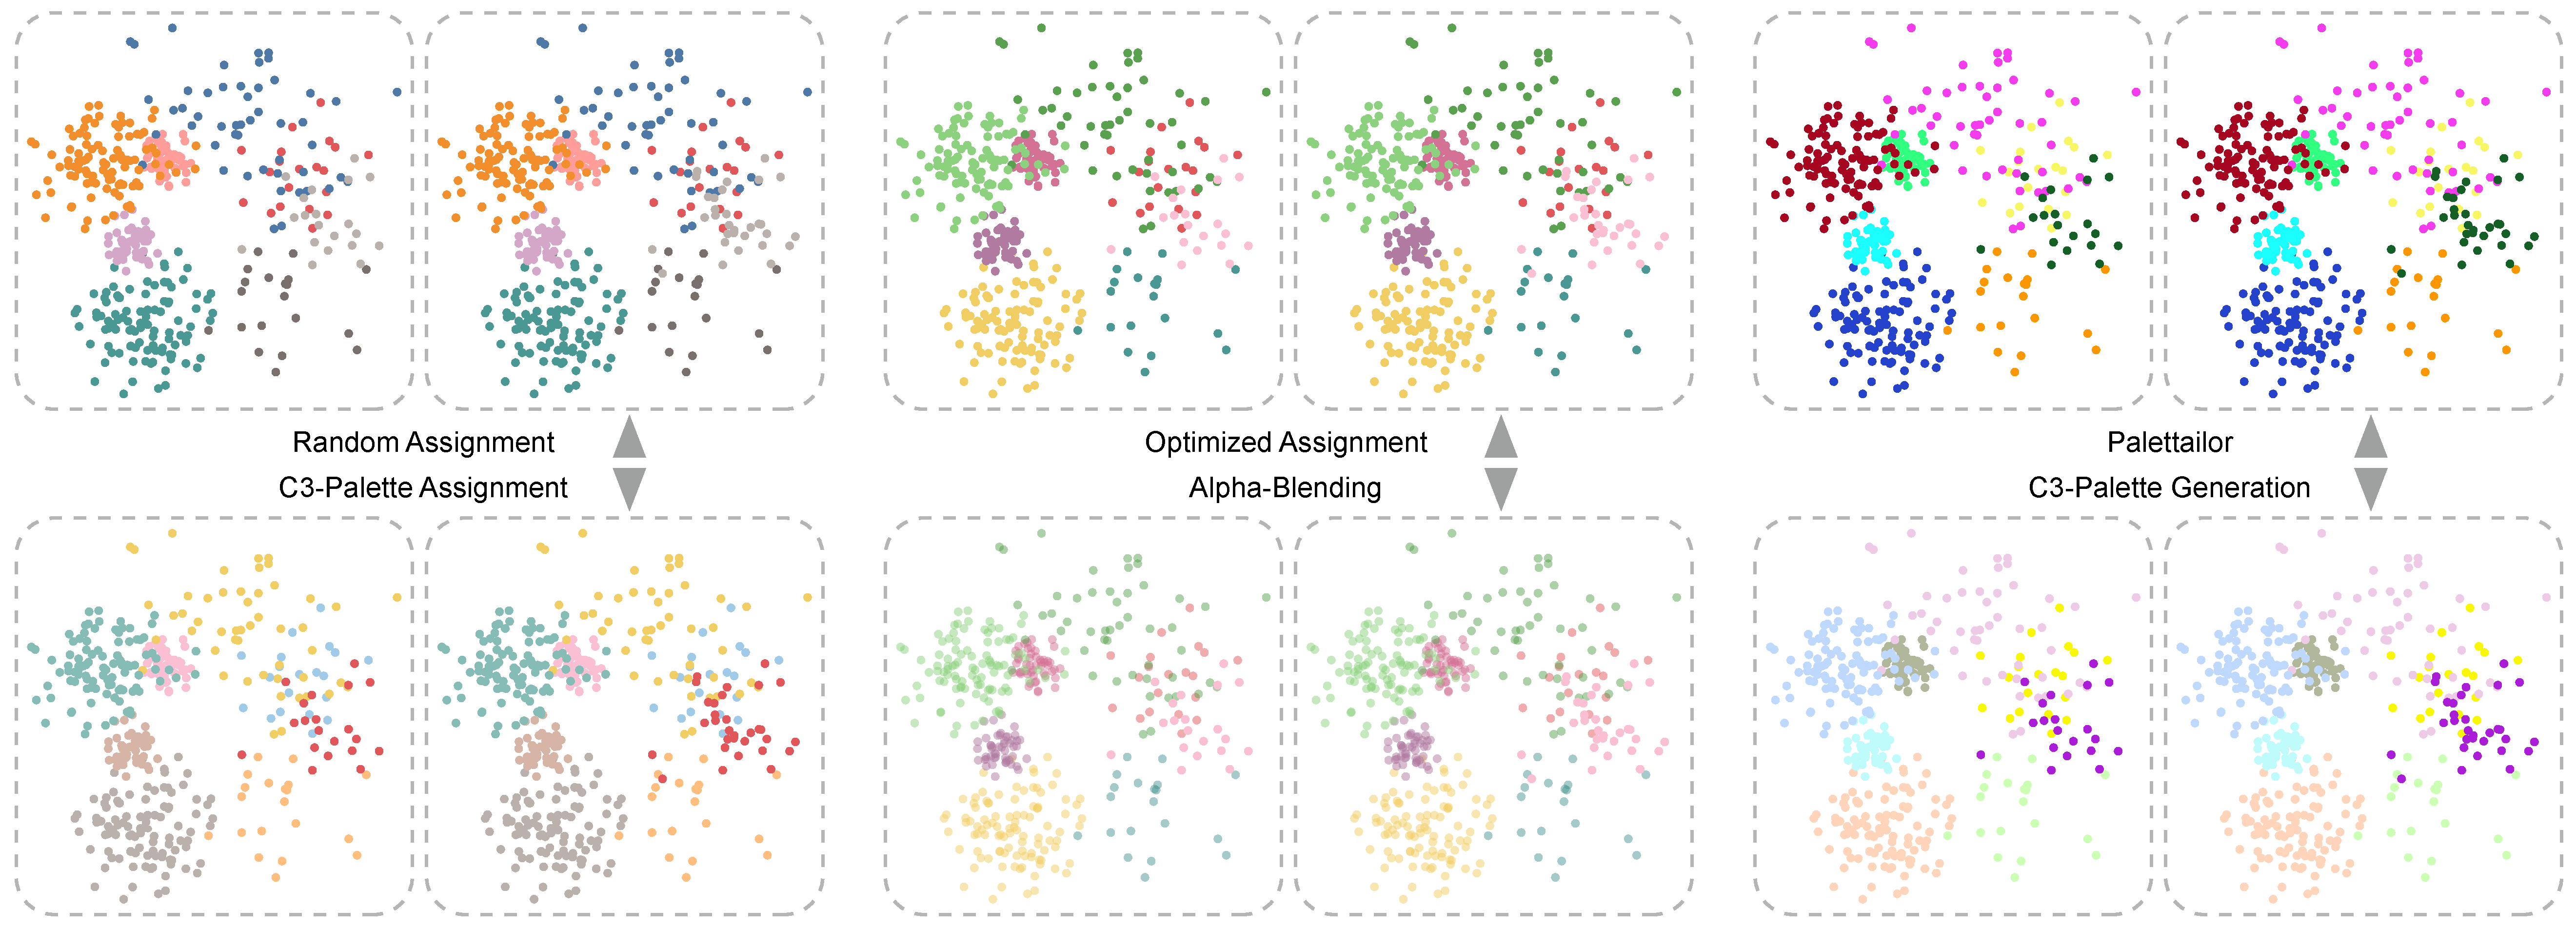
\includegraphics[width=\textwidth]{teaser}
  \caption{Results for different conditions of two categorical scatterplots comparison: (left top) Random Assignment; (left bottom) C3-Palette Assignment; (center top) Optimized Assignment~\cite{Wang2018};
(center bottom) Applying Alpha-Blending on Optimized Assignment, all the classes' alpha are set to 0.5 except the changed class; (right top) Palettailor~\cite{Lu21}; (right bottom) C3-Palette Generation. Our system unifies the palette assignment and palette generation to single or multiple scatterplots in a data-aware manner.}
  \Description{Enjoying the baseball game from the third-base
  seats. Ichiro Suzuki preparing to bat.}
  \label{fig:teaser}
\end{teaserfigure}

%%
%% This command processes the author and affiliation and title
%% information and builds the first part of the formatted document.
\maketitle

\section{Introduction}
ACM's consolidated article template, introduced in 2017, provides a
consistent \LaTeX\ style for use across ACM publications, and
incorporates accessibility and metadata-extraction functionality
necessary for future Digital Library endeavors. Numerous ACM and
SIG-specific \LaTeX\ templates have been examined, and their unique
features incorporated into this single new template.

If you are new to publishing with ACM, this document is a valuable
guide to the process of preparing your work for publication. If you
have published with ACM before, this document provides insight and
instruction into more recent changes to the article template.

The ``\verb|acmart|'' document class can be used to prepare articles
for any ACM publication --- conference or journal, and for any stage
of publication, from review to final ``camera-ready'' copy, to the
author's own version, with {\itshape very} few changes to the source.

\section{Co-Saliency based Color Design}
Given $N$ ($N\geq 2$) categorical visualizations with the same class labels (or a subset thereof), the $j$th visualization has $M$ classes and $n_j$ data items $\{\mathbf{x}^j_1, \cdots, \mathbf{x}^j_{n_j}\}$, where each $\mathbf{x}^j_t$ has a label
$l(\mathbf{x}^j_t)$ and the $i$-th class (with $n^j_i$ data points) consists of $\{\mathbf{x}_{i,1}^j, \cdots , \mathbf{x}_{i,n^j_i}^j\}, i \in  \{ 1, \cdots, m \} $.
For standard bar and line charts, $M$ is equal to $n_j$ but it is often smaller than $n_j$ for scatterplots.
All visualizations use the same  background color $\mathbf{c}_b$ and the same color mapping scheme $\tau: L \mapsto c$. Our goal is to find the best mapping $\tau$ that supports an effective comparison of multiple categorical \od{visualizations}.
% scatterplots.

In line with the design requirements for natural image comparison and categorial data visualization~\cite{Jacobs10,Gleicher18,Lu21},
%~\cite{itti1998model,cheng2014global,zhang2018review},
our problem is formulated based on the following three design requirements:
\begin{enumerate}[label=(\roman*),nosep]
\item \textbf{DR1:} highlighting the most concerned classes between visualizations as much as possible for an efficient comparison;
\item \textbf{DR2:} maximizing the visual discrimination between classes in the individual visualizations for an efficient exploration of multi-class data; and
\item \textbf{DR3:} providing flexible interactions for the exploration of relationships among the compared datasets.
%co-salient classes should follow the principles of visual salience in individual visualizations so that the co-salient classes can be easily identified.
\end{enumerate}
Although visual comparison is an essential part of interactive data analysis, most of  the existing  colorization techniques~\cite{Gramazio17, Lu21} attempt to meet DR2. The key challenge in meeting DR1 is that we need a proper model to characterize the most salient features in multiple visualizations.
To address this issue, we propose our %a categorical visualization
co-saliency model that calculates the saliency of each data item in the context of other similar visualizations. Integrating this model into the objective of a state-of-the-art color mapping generation framework~\cite{Lu21}, we can
generate proper color mappings that highlight salient differences between juxtaposed categorical visualizations while fostering a better visual discrimination of classes.

\subsection{Co-saliency for Multi-class Scatterplots }
Following the definition of image co-saliency~\cite{Jacobs10}, we model class co-saliency with two factors: class importance between visualizations and class contrast within visualizations. The class importance describes how much each class should stand out from the visualization.
Class contrast describes how much each class stands out from neighboring classes and the background,
which is similar to perceptual class separability~\cite{Aupetit02,Wang2018}. Hence,
we define two types of class contrasts: a local contrast with neighboring classes and a contrast with the background.

Since point-based representations are very general in 2D visualization, we use two ($M=2$) horizonally juxtaposed scatterplots to illustrate our method.
Analogous to bottom-up image co-saliency models~\cite{Jacobs10,Fu13}, the co-saliency of the $i$th class is defined as the product between the class importance and  class contrast scores to emphasize the target class and the co-saliency for $M$ classes:
\begin{equation}
% E_{CoS} = \sum_i   \sum_j (1-\lambda) \alpha^j_i  \exp(\theta_i) + \lambda \beta_i  f(\theta_i)
E_{CoS} = \sum_i^M    \left(\sum_j^N \frac{1}{n^j_i}\bigg(\lambda \alpha^j_i\exp(\theta_i) + (1-\lambda) \beta^j_i f(\theta_i) \bigg) \right)
	\label{eq:cosaliency}
\end{equation}
where $\theta_i$ is the importance of the $i$th class,
$n^j_i$ is the number of points of the $i$th class in the $j$th scatterplot,
$\alpha^j_i$ is the local contrast with the neighboring classes of the $i$th class in the $j$th scatterplot, $\beta^j_i$  is the contrast of the class to the background, and $\lambda$ is the weight between them. The weight $1/{n^j_i}$  is used to alleviate class imbalances  so that  classes with small numbers of points and large changes can be highlighted.

To better support DR1, we apply an exponential function to enlarge the weight of structural class changes, while using a piecewise function weighting the background contrast:
\begin{align}
f(\theta_i) =  \left\{ \begin{array}{ll}
\exp(\theta_i) & \textrm{if $\theta_i>\kappa$}\\
-\exp(\theta_i) & \textrm{else}
\end{array} \right.
\label{eq:energyfunc}
\end{align}
$\kappa$ is a user-specified threshold with a default of zero. The reason for the two different weighting schemes is that classes with less or no changes might be treated as the background by viewers~\cite{zhang2018review}. To suppress the saliency of such classes, we introduce a negative importance for them.

\vspace{2mm}
\noindent\textbf{Local Contrast}.
%Given the $j$th scatterplot, we define the local class contrast based on the point distinctness~\cite{Lu21}.
%Here, we briefly describe its computation process and
%refer to Lu et al.~\cite{Lu21} for more details.
%Given the data point $\mathbf{x}^j_t$, its distinctness is defined as the sum of the color differences from its neighbourhoods weighted by the inverse Euclidean distance.
%Then, the distinctness of the $i$th class is the sum of all points with the same class label in the scatterplot, which is further normalized by ${n^j_i}$.
Given the $j$th scatterplot, we define the local class contrast based on the $\alpha$-shape based point distinctness~\cite{Lu21}.  For each data point $\mathbf{x}^j_t$, we define its point distinctness  as:
\begin{align}
 \gamma (\mathbf{x}^j_t)=\frac{1}{|\Omega^j_t|} \sum_{\mathbf{x}^j_p \in \Omega^j_t}  \frac{\Delta\epsilon(\tau(l(\mathbf{x}^j_t)),\tau(l(\mathbf{x}^j_p)))}{d(\mathbf{x}^j_t,\mathbf{x}^j_p)} \nonumber ,
\end{align}
where $\Omega^j_t$ is set of $k$ nearest neighbors of $\mathbf{x}^j_t$, $\tau(l(\mathbf{x}^j_p))$ is the color of $\mathbf{x}^j_p$,  $d$ is the Euclidean distance and $\Delta\epsilon$ is the CIELAB color distance.
For the $i$th class, its local contrast is the sum of all points with the same class label in the scatterplot:
\begin{align}\label{eq:nc}
 \phi^j_i = \frac{1}{n_j}\sum^{n_j}_{p}\gamma(\mathbf{x}^j_p) \delta(l(\mathbf{x}^j_p),i)
\end{align}
where $\delta(l(\mathbf{x}^j_p),i)$ is one if the class label $l(\mathbf{x}^j_p)$ is $i$ and else zero.

If a class overlaps with different classes, the local contrast value will be high and the value will be small for a well separated class. Hence, the black class  in the  two scatterplots shown in Fig.~\ref{fig:map}(a)  has a low contrast value (see Fig.~\ref{fig:map}(b)) and the cyan class has a large value.


%\begin{align}\label{eq:pdc}
% \alpha^j_i = \frac{1}{n^j_i}\sum^{n_j}_{p}\gamma(\mathbf{x}^j_p) \delta(l(\mathbf{x}^j_p),i)
%\end{align}
%where $\delta(l(\mathbf{x}^j_p),i)$ is one if the class label $l(\mathbf{x}^j_p)$ is $i$ and else zero.
%
%
%However, KNNG cannot reflect the contrast among classes without any overlap. For example,  in Fig.~\ref{fig:knng}(a) the contrast between the blue class and the brown classes cannot be reflected.
%To address this issue, we introduce an additional class-center based contrast cue~\cite{Fu13}.
%Suppose the center of the $i$th class in this scatterplot is $\mu^j_i$, the class contrast is:
%\begin{align}\label{eq:cc}
% \varphi^j_i =  \frac{1}{M}\sum^M_{m}\frac{\Delta\epsilon(\tau(i),\tau(m))}{||\mu^j_m -\mu^j_i ||},
%\end{align}
%which assigns large weights to nearby classes and small ones to far-away classes. The final class contrast of the $i$th class is:
%\begin{align}\label{eq:pd}
% \alpha^j_i  = \phi^j_i  + \omega \varphi^j_i,
%\end{align}
%where the weight $\omega$ is 1.0 in our experiment.

\vspace{2mm}
\noindent\textbf{Background Contrast}.
The contrast with the background is based on the \od{so-called} point non-separability $\rho (\mathbf{x}^j_t)$ (rf.~\cite{Wang2018}), which is defined as the difference between two  separation degrees:
\begin{align}
\rho(\mathbf{x}^j_t)&= b(\mathbf{x}^j_t)-a(\mathbf{x}^j_t) \ .
\end{align}
where $b(\mathbf{x}^j_t)$ is the between-class separation degree and $a(\mathbf{x}^j_t)$ is the within-class separation degree.
% of $\mathbf{x}^j_t$.
\od{The measures are defined as weighted sums of  color differences of $\mathbf{x}^j_t$ with its neighborhood from the same and different classes:}
\begin{align}
a(\mathbf{x}^j_t)&=\frac{1}{|\Omega^j_t|}\sum_{\mathbf{x}^j_p \in \Omega^j_t } \frac{\delta(l(\mathbf{x}^j_t), l(\mathbf{x}^j_p))
\Delta\epsilon(\tau(l(\mathbf{x}^j_t)),\mathbf{c}_b)
}{d(\mathbf{x}^j_t,\mathbf{x}^j_p)} , \;\;
b(\mathbf{x}^j_t)=\frac{1}{|\Omega^j_t|}\sum_{\mathbf{x}^j_p \in \Omega^j_t } \frac{1-\delta(l(\mathbf{x}^j_t), l(\mathbf{x}^j_p))\Delta\epsilon(\tau(l(\mathbf{x}^j_t)),\mathbf{c}_b)}{d(\mathbf{x}^j_t,\mathbf{x}^j_p)}  \nonumber
\end{align}

When most neighbor points of $\mathbf{x}^j_t$ have the same label as $\mathbf{x}^j_t$,  $\rho (\mathbf{x}^j_t)$ is negative.
% and vice versa.
%the corresponding class has large within-class separability and small between-class separability and thus $\rho (\mathbf{x}^j_t)$ is negative; and vice versa.
However, such a negative $\rho (\mathbf{x}^j_t)$ makes the optimization in Eq.~\ref{eq:cosaliency} meaningless, \od{and the corresponding} classes might be highlighted no matter how large the change of this class is.
\od{To address this issue, we use an exponential function to let $\rho (\mathbf{x}^j_t)$  always be positive while maintaining the monotonicity of the function.} Accordingly, we define
%\begin{align}\label{eq:ctb}
% \rho (\mathbf{x}^j_t)=\frac{1}{|\Omega^j_t|} \sum_{\mathbf{x}^j_p \in \Omega^j_t}  \frac{(1-2\delta(l(\mathbf{x}^j_t),l(\mathbf{x}^j_p)))\Delta\epsilon(\tau(l(\mathbf{x}^j_t)),\mathbf{c}_b)}{d(\mathbf{x}^j_t,\mathbf{x}^j_p)} ,
%\end{align}
the contrast to the background of the $i$th class as:
\begin{align}\label{eq:ctbc}
 \beta^j_i = \frac{1}{n^j_i}\sum^{n_j}_{t} \exp(\rho(\mathbf{x}^j_t)) \delta(l(\mathbf{x}^j_t),i).
\end{align}
%where
%$\delta(l(\mathbf{x}^j_p),i)$ is one if the class label $l(\mathbf{x}^j_p)$ is $i$ and else zero.
%In doing so, all classes have positive background contrast value.
As illustrated in Fig.~\ref{fig:map}(c), well-separated classes with large color differences from the background have large background contrast (blue and black classes), whereas the pink and cyan classes have relatively large background contrast values with a medium class separation.


%\begin{wrapfigure}{r}{0.28\columnwidth}
%	\vspace{-5mm}
%	\centering
%	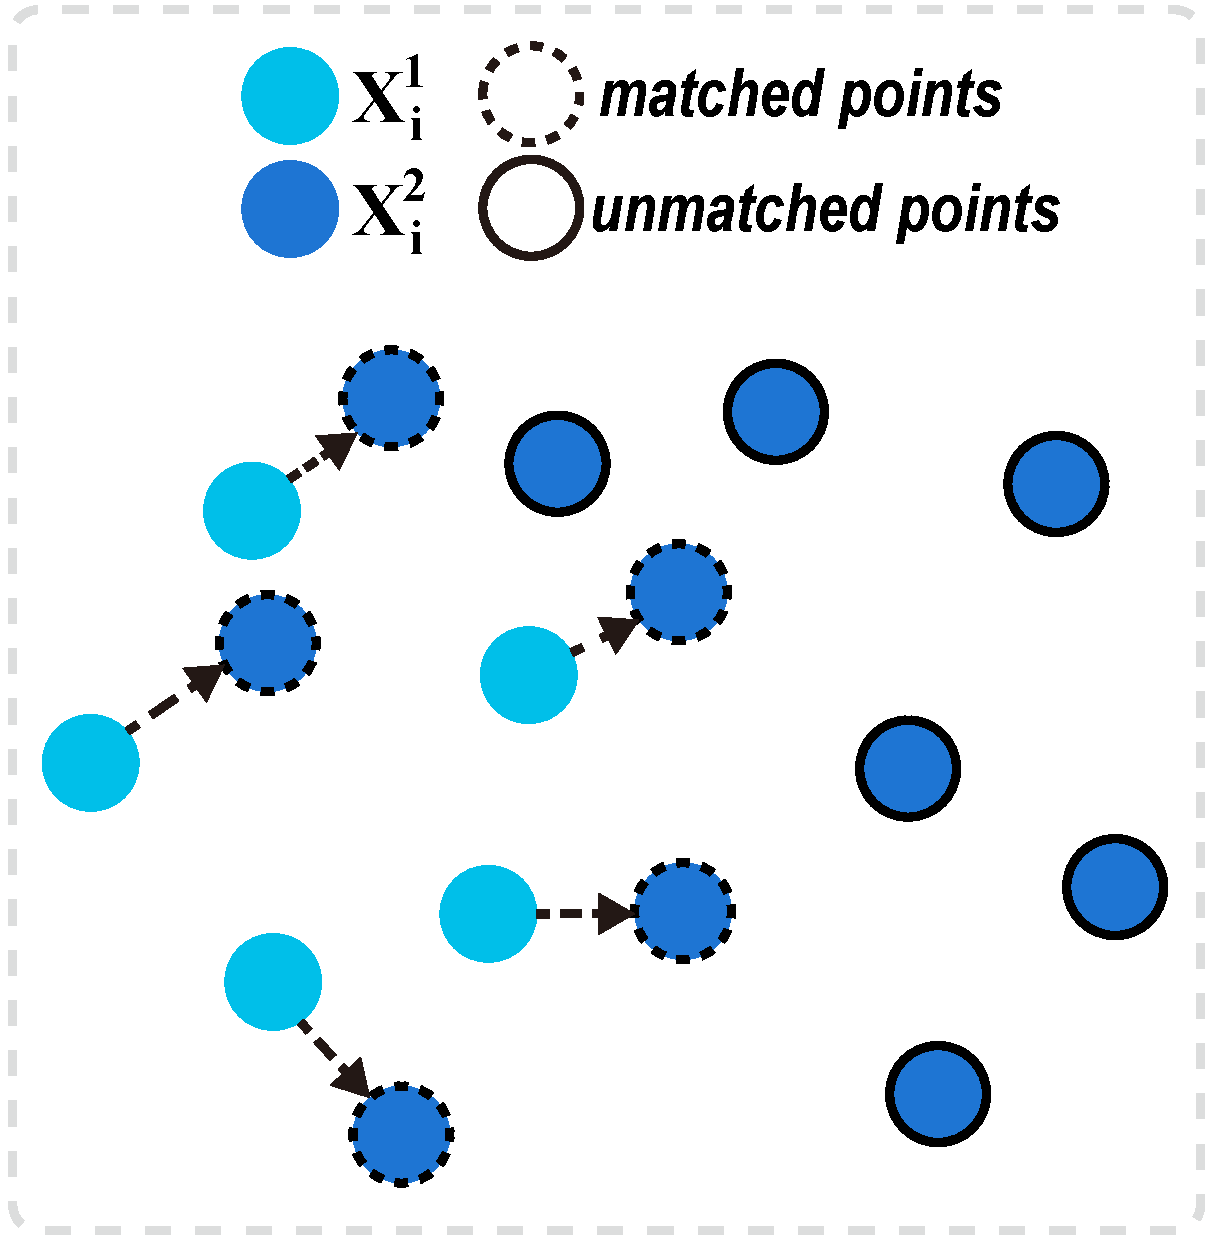
\includegraphics[width=0.28\columnwidth]{class-change-degree}
%	\vspace*{-8mm}
%	\caption{An one-to-one mapping for computing the changes between two classes.}
%	\vspace*{-2mm}
%	\label{fig:class-change-degree}
%\end{wrapfigure}
 %Since $\rho (\mathbf{x}^j_t)$ might be a negative value which will be influenced by Eq.~\ref{eq:piecewiseFunc}, we apply an exponential function to transfer it to positive while maintains the monotonicity.

\vspace{1.5mm}
\noindent\textbf{Class Importance}.
Class importance reflects whether a class should be highlighted or not. It can be specified by user or by some measures. In our paper, as a default we use the class change degree to represent the importance of each class.
To quantify how users perceive structural changes of classes, we measure the difference between the class distributions in two scatterplots using the Earth Mover's Distance (EMD)~\cite{rubner2000earth}, a perceptual metric.
Suppose the $i$th  class with two \od{representations by two} sets of points $\mathbf{X}^1_i = \{\mathbf{x}_{i,1}^1, \cdots , \mathbf{x}_{i,n^1_i}^1\}$ and $\mathbf{X}^2_i = \{\mathbf{x}_{i,1}^2, \cdots , \mathbf{x}_{i,n^2_i}^2\}$.
Taking the Euclidian distance between points as the cost, we need to  minimize the total matching cost
\begin{align}
 H(\mathbf{X}^1_i, \mathbf{X}^2_i)  = \min_\chi \sum_t d(\mathbf{x}_{i,t}^1, \mathbf{x}_{i,\chi(t)}^2), \nonumber
\end{align}
which constrains one-to-one mappings $\chi$ between points %(see an illustration in Fig.~\ref{fig:class-change-degree}).
This is the classic bipartite matching problem, which can be solved by the Hungarian method~\cite{kuhn1955hungarian}.
When the number of points of two sets is not equal, we further take the difference between the number of points into account. \od{In doing so, the class change degree contains  positional changes and changes of element numbers:}
\begin{align}\label{eq:cm}
 \theta_i= \frac{H(\mathbf{X}^1_i, \mathbf{X}^2_i) }{\min\{n^1_i, n^2_i\}} + \nu \frac{||n^1_i- n^2_i||}{\max\{n^1_i, n^2_i\}}
\end{align}
both terms range within [0,1] and $\nu$ is 1.0 as default value.


\begin{figure*}[!tb]
\centering
\includegraphics[width=\linewidth]{figures/saliencymap}
\caption{Main components for computing co-saliency maps: For the two input scatterplots (a), our class-based co-saliency (e) is generated by fusing  local contrast (b),  background contrast (c),  and class change degree (d). Brightness of points denotes value.
	% and vice versa.
}
\vspace*{-3mm}
\label{fig:map}
\end{figure*}
\vspace{1.5mm}

Fig.~\ref{fig:map} shows an example of two 8-class scatterplots with three  changing classes (orange, blue and black). Combining the class change degree with the two above-given contrast measures allows us to highlight salient differences and maintain the visual discrimination of the classes (see Fig.~\ref{fig:map}(e)).

\subsection{Co-Saliency based Color Mapping}
\label{subsec:solver}
On the basis of the co-saliency model, we meet DR1 and DR2 in two ways: co-saliency based color assignment and co-saliency based palette generation.

\vspace{1.5mm}
\noindent\textbf{Co-saliency based Color Assignment}.
Given a good color palette with $P$ colors ($P\geq M$), the optimal color mapping can be obtained by
taking the co-saliency model in Eq.~\ref{eq:cosaliency} as the objective of the state-of-the-art color assignment method~\cite{Wang2018}. Starting from a random permutation of $P$ colors, we use the simulated annealing algorithm~\cite{aarts1989stochastic} to find the optimal permutation with two randomized strategies to improve the solution. One is randomly exchanging two colors from the selected $m$ colors and the other is replacing one color from the $m$ selected colors with the one chosen from the unselected $P-M$ colors. With a few iterations, we can obtain a reasonable color mapping as shown in Fig.~\ref{fig:teaser} bottom left.

\begin{figure}[h]
\centering
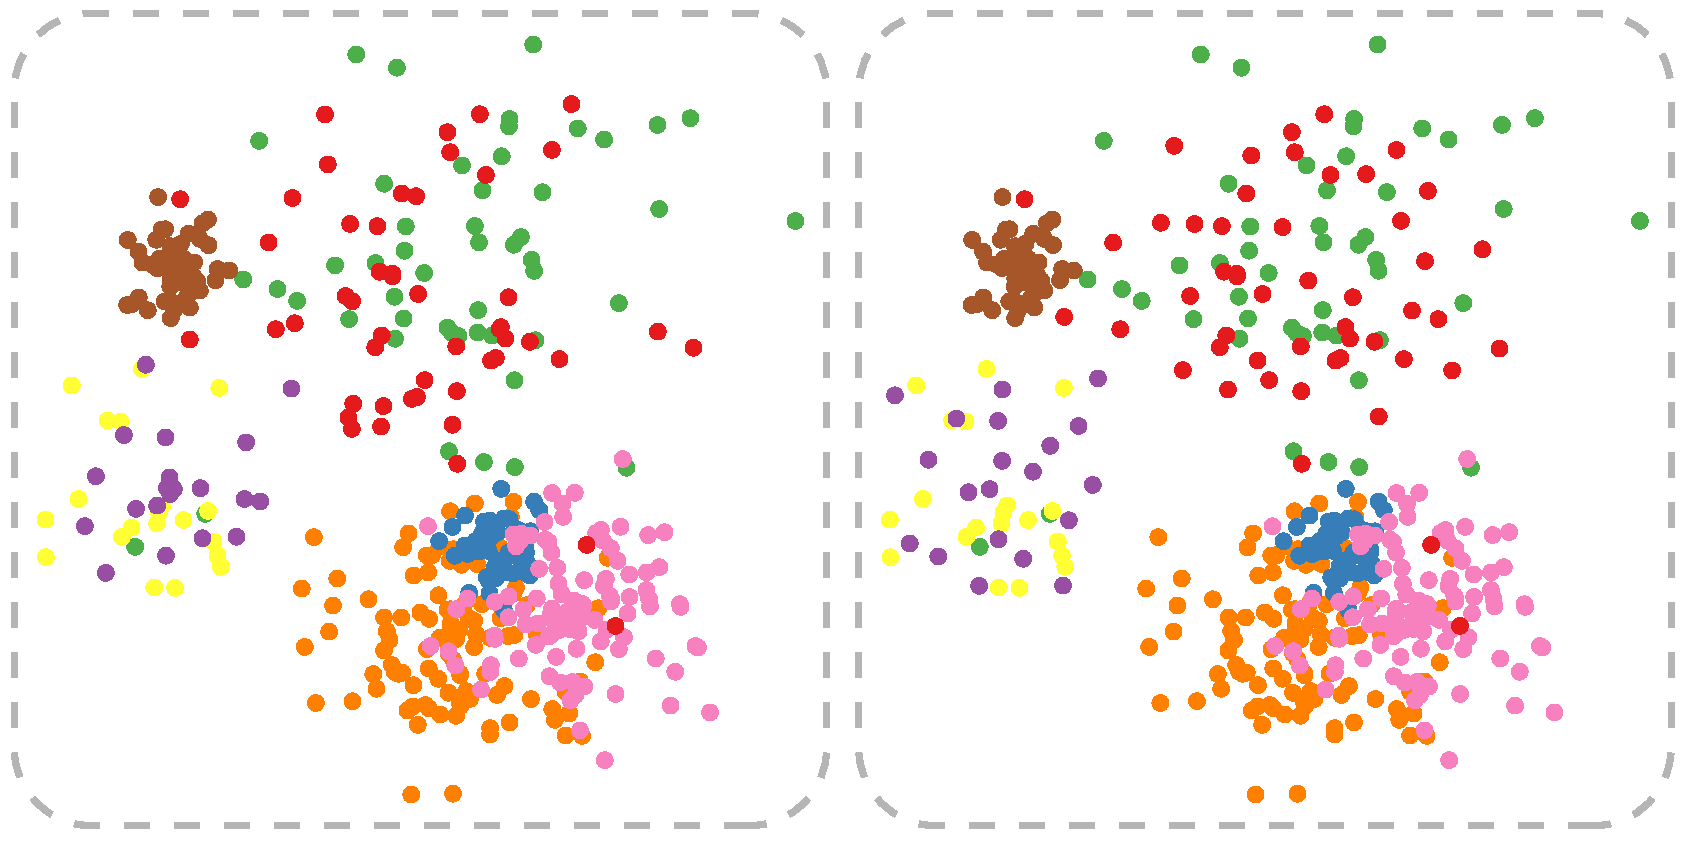
\includegraphics[width=.8\columnwidth]{figures/colorbrewer.pdf}
\caption{Visualizing the same data sets as shown in Fig.~\ref{fig:lambda} with the ColorBrewer palette and our assignment method.}
\vspace*{-3mm}
\label{fig:colorbrewer}
\end{figure}

However, this method has two major limitations: i) requiring users to try many palettes for selecting a good one; and ii) the design of most existing palettes is not oriented towards visual comparison so that even the best color assignment cannot provide prominent cues for this task.
%For example, all colors in the Tableau palette are highly discriminable and it is hardly to find a satisfactory solution, see Fig.~\ref{fig:teaser} (b). Thus, we prompt users to use our co-saliency based palette generation method.
For example, all colors in the ColorBrewer 8-class Set1~\cite{harrower2003colorbrewer} palette are highly discriminable, but it is hard to find a satisfactory solution. Fig.~\ref{fig:colorbrewer} shows an example, where the change of the red class is hard to identify at once even it is very distinctive. Thus, we prompt users to use our co-saliency based palette generation method.


\vspace{1.5mm}
\noindent\textbf{Co-saliency based Palette Generation}.
The recently proposed data-aware palette generation method~\cite{Lu21} automatically generates discriminable and preferable palettes by maximizing the combination of three palette quality measures: point distinctness, name difference, and color discrimination.
By replacing the first measure with our co-saliency model, the palette generation is formulated as an optimization problem:
\begin{equation}
\arg\max_{\mathbf{\tau}} E(\mathbf{\tau}) = \omega_0 E_{CoS} + \omega_1 E_{ND} + \omega_2 E_{CD}.
\label{eq:energyfunc}
\end{equation}
which consists of a co-saliency term $E_{CoS}$ (see Eq.~\ref{eq:cosaliency}), a name difference term $E_{ND}$ and a color discrimination term $E_{CD}$, balanced by $\omega_0$, $\omega_1$ and $\omega_2$. For more detail about $E_{ND}$ and $E_{CD}$, we refer readers to~\cite{Lu21}. By using the same optimization method as Lu et al.~\cite{Lu21}, we can generate desired colors in real time. %see Fig.~\ref{fig:teaser} (d).



\subsection{Parameter Effect}
\label{subsec:parameter}
Besides different weights for different terms in palette generation~\cite{Lu21}, our co-saliency model involves three parameters: the weight $\lambda$ between two contrasts, the threshold for the class importance $\kappa$, and $\nu$ that is related to the definition of the class change degree which is used as our default class importance.
Since $\nu$ is fixed in our experiments and the class importance can be specified by user, we mainly discuss the effects of $\lambda$  and $\kappa$.

\begin{figure}[h]
\centering
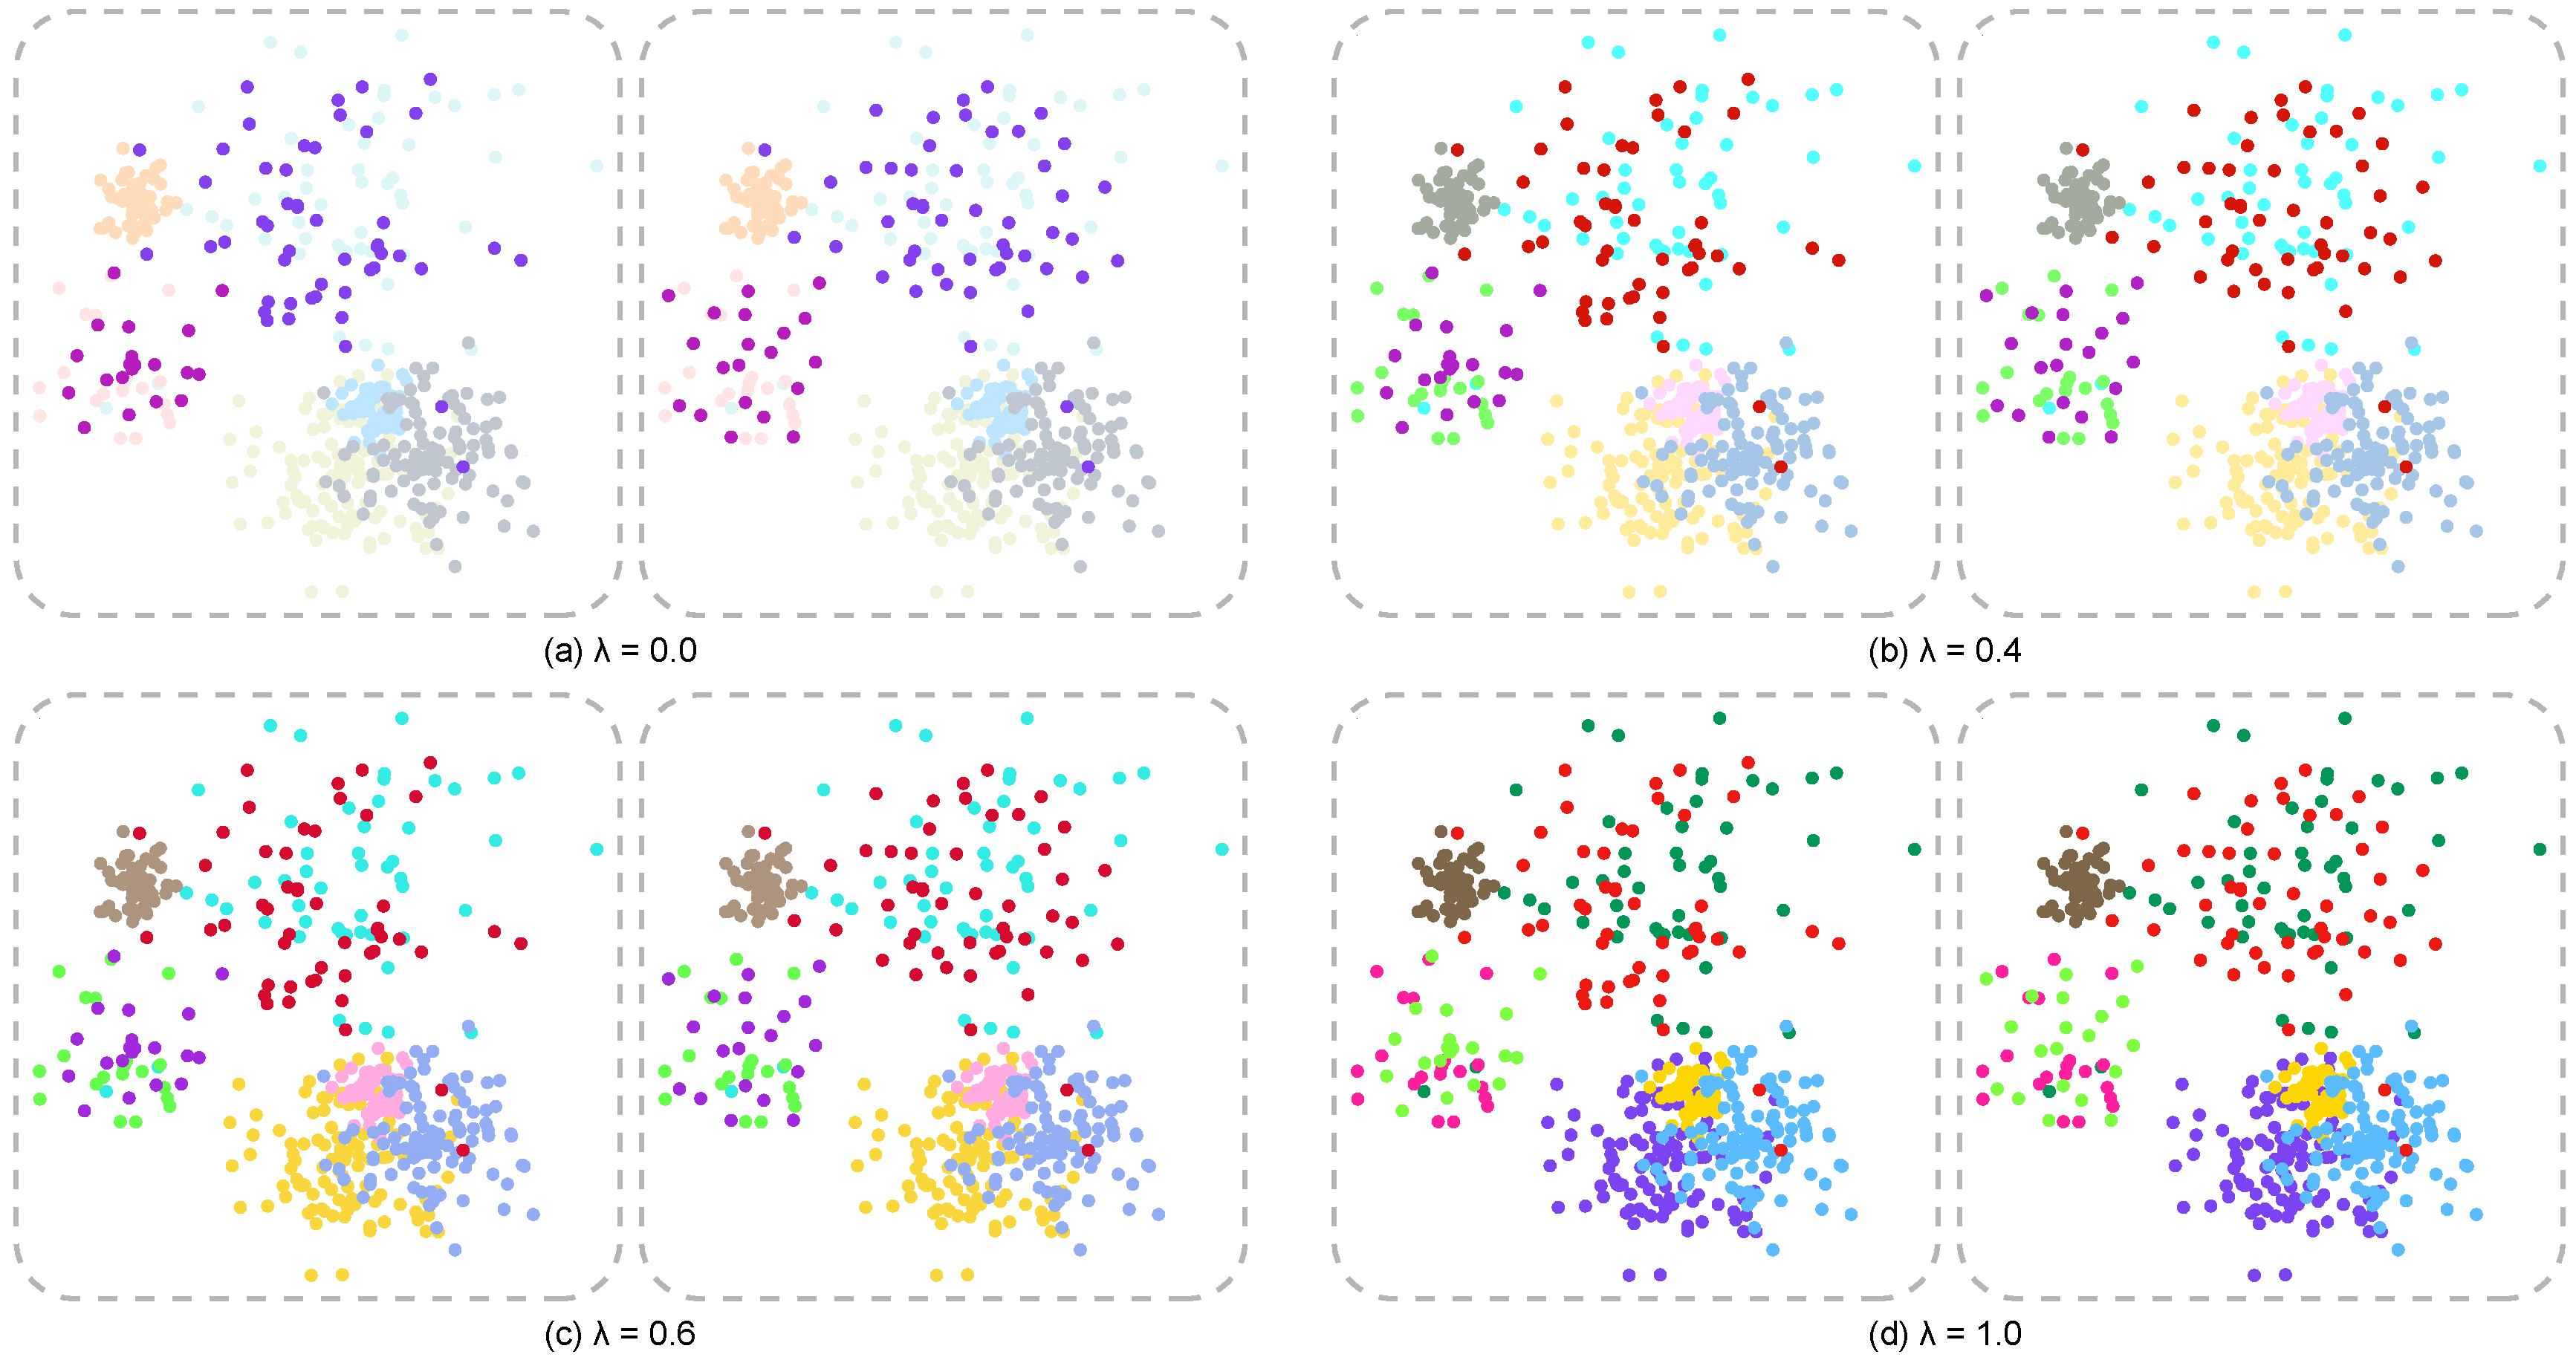
\includegraphics[width=0.8\textwidth]{figures/lambda.pdf}
\caption{Effect of $\lambda$: (a) result generated by only considering contrast to the background; (b) result generated by setting $\lambda$ to 0.4; (c) result generated by setting $\lambda$ to 0.6; (d) result generated by only considering contrast with nearest classes.}
\vspace*{-3mm}
\label{fig:lambda}
\end{figure}
%\vspace{3mm}

\noindent\textbf{Balancing Weight $\lambda$}.
Although this parameter modulates the influence between the class contrast with neighbors and background, it offers a compromise between DR1 and DR2.
As shown in Fig.~\ref{fig:lambda}(a), considering only the contrast to the background would have a good 'pop out' effect but other classes are hard to discriminate. While considering only the contrast with nearest neighbors, such as Fig.~\ref{fig:lambda}(d), all the classes are each to distinguish but the changed classes are hard to find out.
This is reasonable, because pre-attentive vision
% processing mechanism
lets a bright saturated color region within  regions of de-saturated colors ``pop-out'' to the viewer~\cite{healey1995visualizing}.
In our experiments, we found that setting  $\lambda=0.4$ as the default allows to simultaneously emphasize changes and preserve the discriminability between classes, see an example in Fig.~\ref{fig:lambda}(b).


\vspace{1.5mm}
\noindent\textbf{Importance Threshold $\kappa$}.
The threshold $\kappa$ selects the classes with large importance to be highlighted.
With a default value of zero, all classes with importance value larger than zero are ensured to be highlighted. Likewise, a large $\kappa$ will de-emphasize classes with a small importance.
We further allow users to specify $\kappa$ by interaction through the control panel (see Sec.~\ref{sec:interaction}).

\begin{figure}[h]
\centering
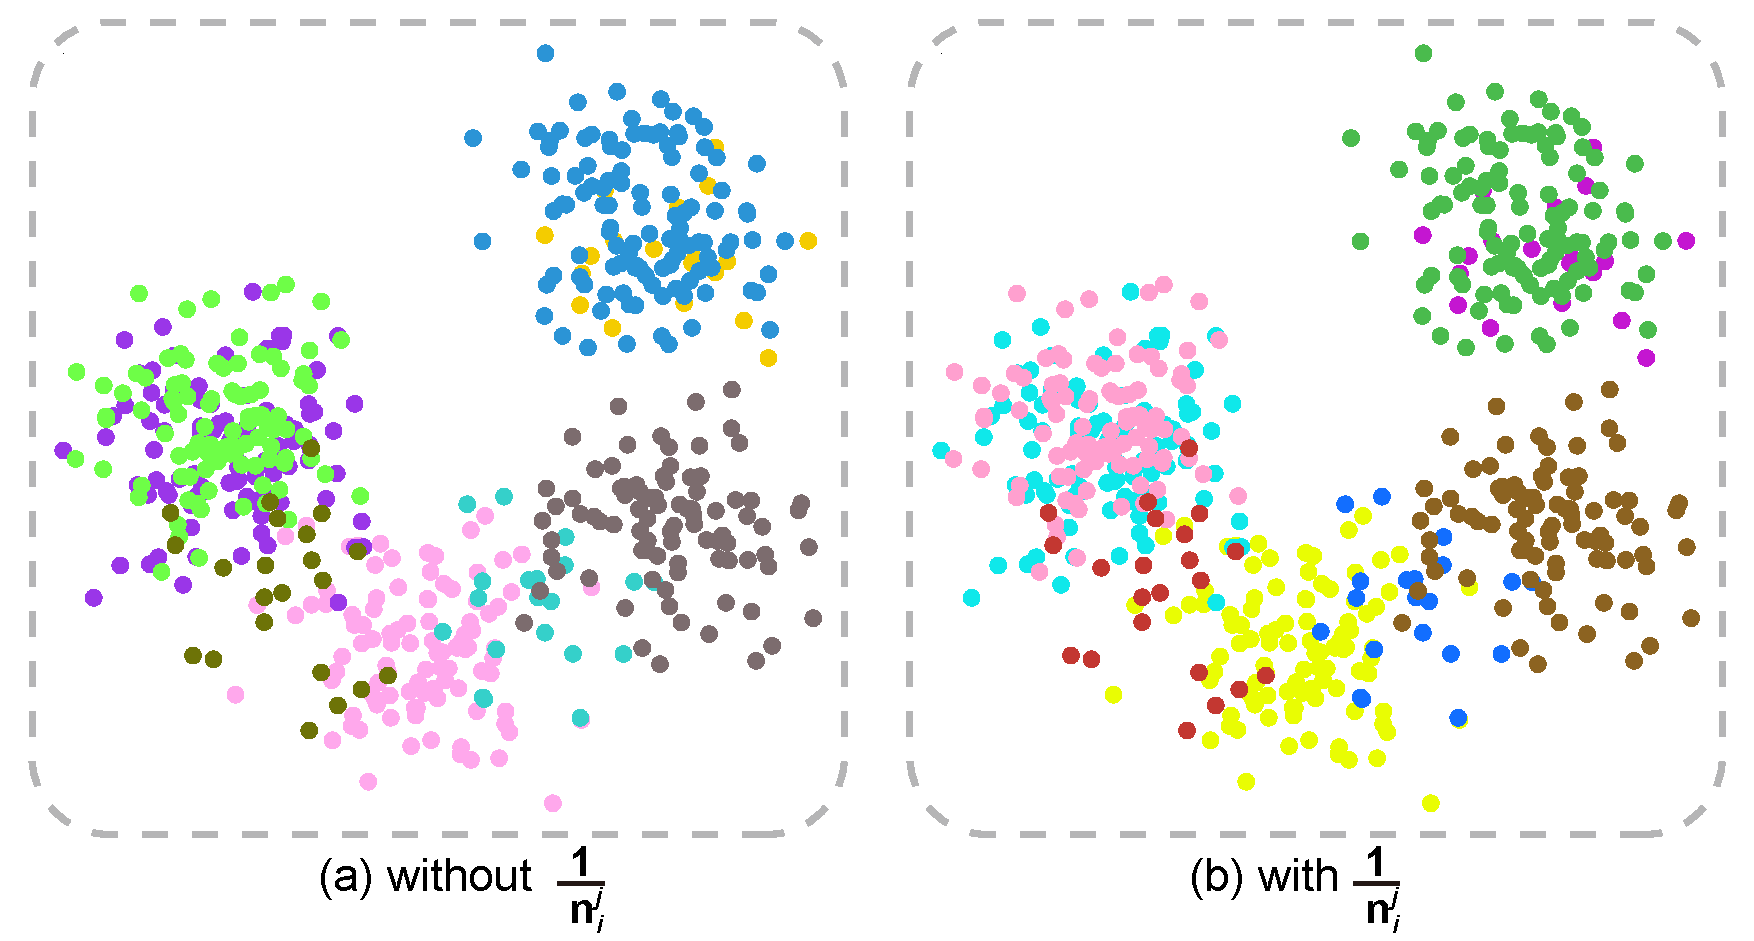
\includegraphics[width=0.8\textwidth]{figures/nij.pdf}
\caption{Effect of $\frac{1}{n^j_i}$: (a) without this term the small classes are hard to catch user's attention; (b) with this term, small classes are easy to find. Palettes are generated with same scatterplot.}
\vspace*{-3mm}
\label{fig:nij}
\end{figure}
%\vspace{.5em}

We can observe that when there's only one scatterplot and $\theta_i$ of each class is zero, then Equation.~\ref{eq:cosaliency} is very similar to the objective function of ~\cite{Wang2018}. Our method extends Wang et.al's work to multiple scatterplots with a carefully designed co-saliency model. Besides, we add $\frac{1}{n^j_i}$ to emphasize the class with less points. As shown in Fig.~\ref{fig:nij}(b), with this new term, the little classes, like red, blue and purple classes, become more discriminable.


\begin{figure}[ht]
\centering
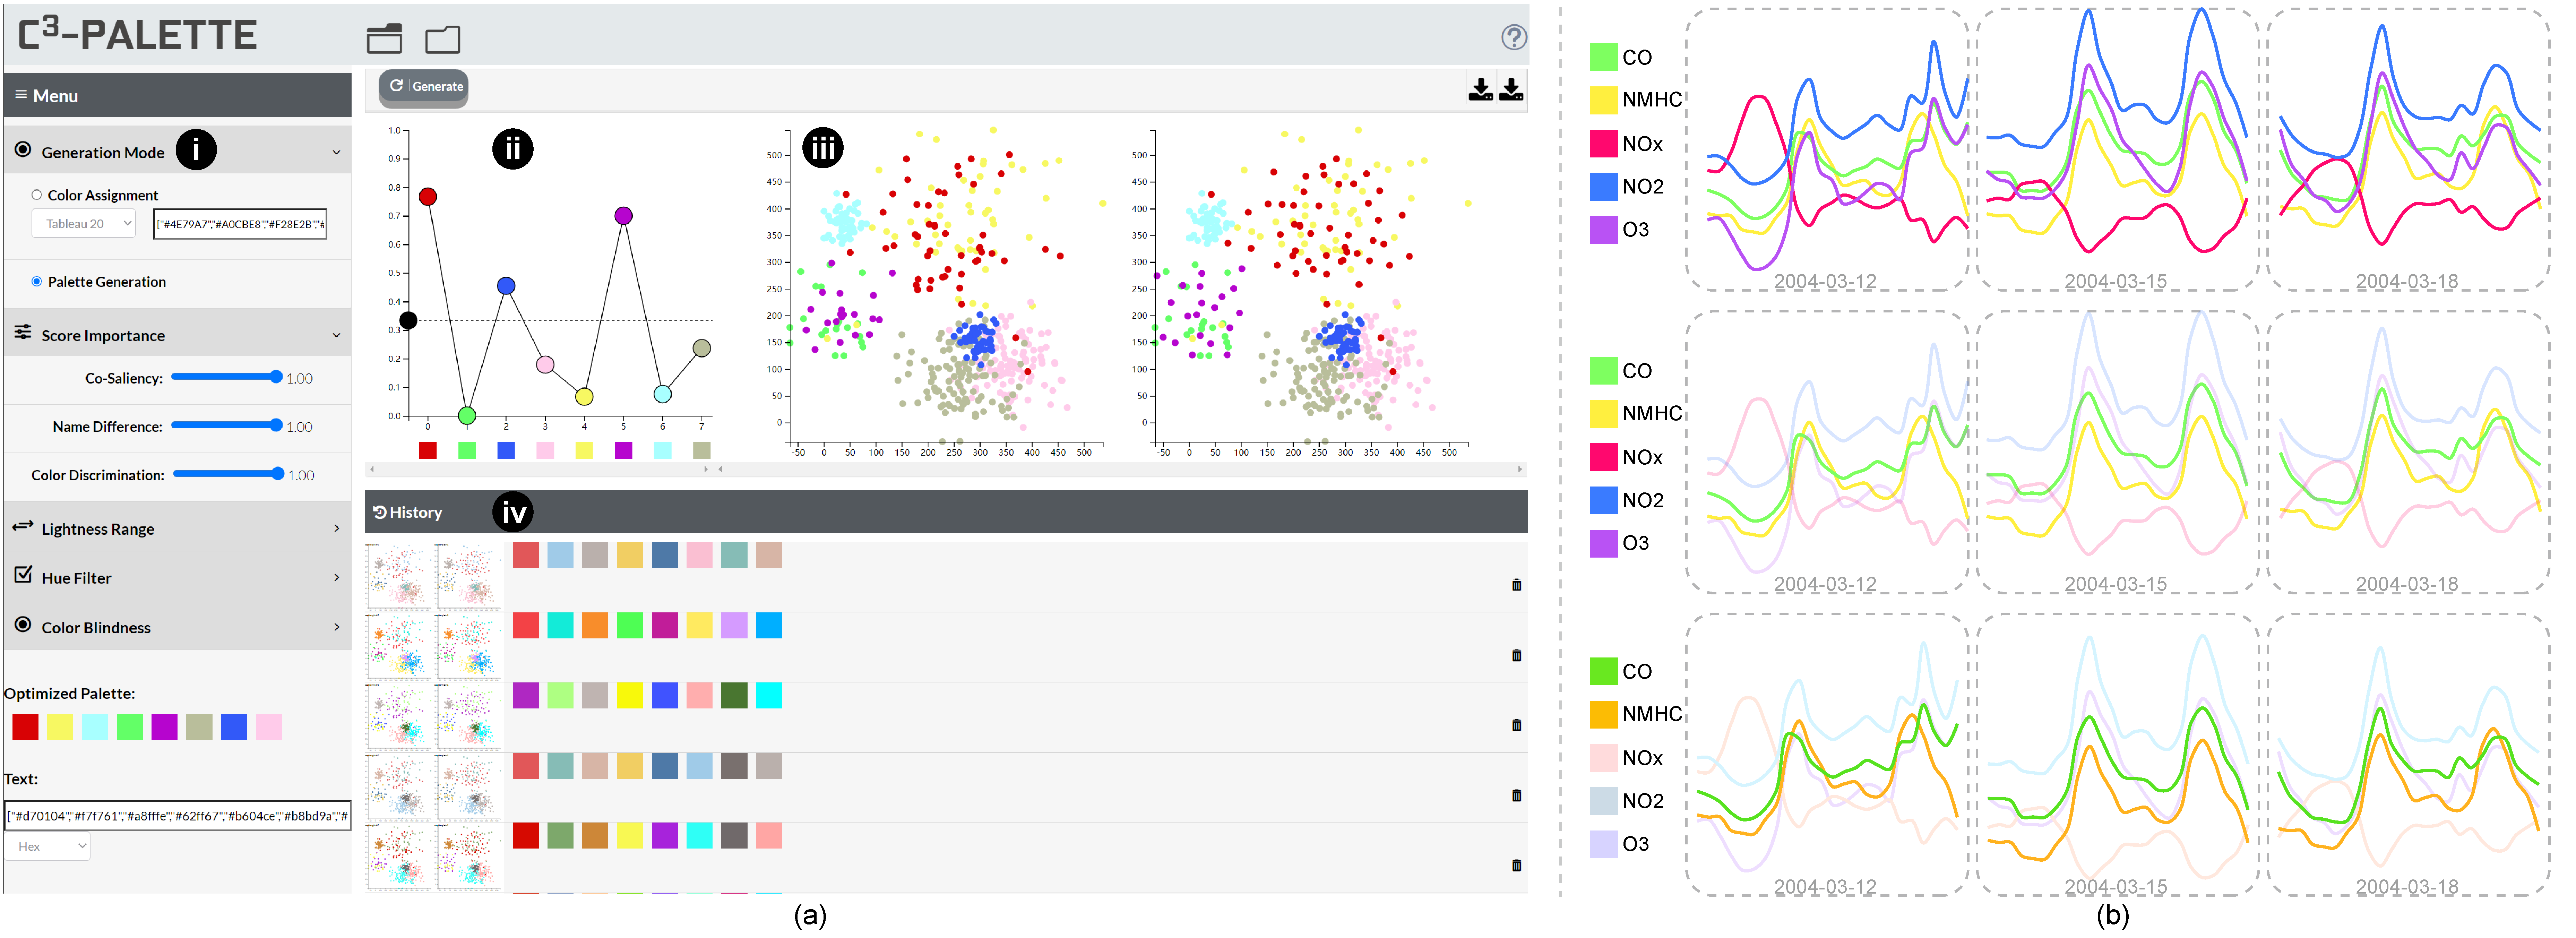
\includegraphics[width=0.8\columnwidth]{figures/interface-linechart.pdf}
\caption{(a) Screenshot of the interactive system consisted of four panels: (1) Settings Panel; (b Control Panel; (3) Visualization Panel; and (4) History Panel. (b)}
\vspace*{-3mm}
\label{fig:ui}
\end{figure}

\section{Interactive System}
\label{sec:interaction}
To help users interactively design colors for comparing multi-class scatterplots, we developed a web-based multi-view visualization tool \footnote{\small \url{https://c3-palette.github.io/}} (see Fig.~\ref{fig:ui}).
It consists of four coordinated views: (a) a settings panel, (b) a control panel for adjusting importance threshold $\kappa$ and even importance value of each class, (c) the juxtaposed visualizations, and (d) a history view. The control panel shows the decision which classes are highlighted, and the history view allows to quickly explore and access previous color mappings.

After uploading multiple categorical scatterplots, the user can either choose a default color palette or use our system to automatically generate color palettes. In this case, the system automatically finds an optimal color mapping scheme to colorize the input data, while each class is encoded as a circle where the x-axis represents class label and the y-axis indicates the importance of each class. By default, the importance is represented by the change degree and $\kappa$ is set to zero. User can drag the circle to modify the corresponding importance value. The $\kappa$ is controlled by a black circle on the y-axis which can also be dragged to modify. Our system finds a color mapping scheme to highlight the classes with large importance and renders the classes in ascending order of the corresponding importance. If users like the color mapping scheme, they can save it to the history view.

\vspace{1.5mm}
\noindent\textbf{Flexible Importance Manipulation}.
Using $\theta_i$  defined in Eq.~\ref{eq:cosaliency}, the classes whose importance values are larger than the threshold $\kappa$ will be highlighted.
Fig.~\ref{fig:ui}(b,c) show an example, where the three classes with the adjusted importance values larger than $\kappa$ are emphasized with salient \emph{red}, \emph{blue} and \emph{purple} colors, respectively.
This control panel allows users to select arbitrary classes of interest to highhlight by simply adjust circle position and $\kappa$ value. More use cases can be seen in Sec.~\ref{sec:caseStudy}.

\vspace{1.5mm}
\noindent\textbf{Color Vision Deficiency}.
To help people with a color vision deficiency, we allow users to generate palettes that can be used for different types of vision problem, such as protanomaly and deuteranomaly which result in poor red-green hue discrimination. This is achieved by adopting a color blindness simulator(the source code can be find at github: https://github.com/MaPePeR/jsColorblindSimulator) and then used our matrix for palette evaluation. Fig.~\ref{fig:blindness} show an example, where the left two images show the auto-generated results and the right are the simulated results perceived by people with protanomaly.

\begin{figure}[ht]
\centering
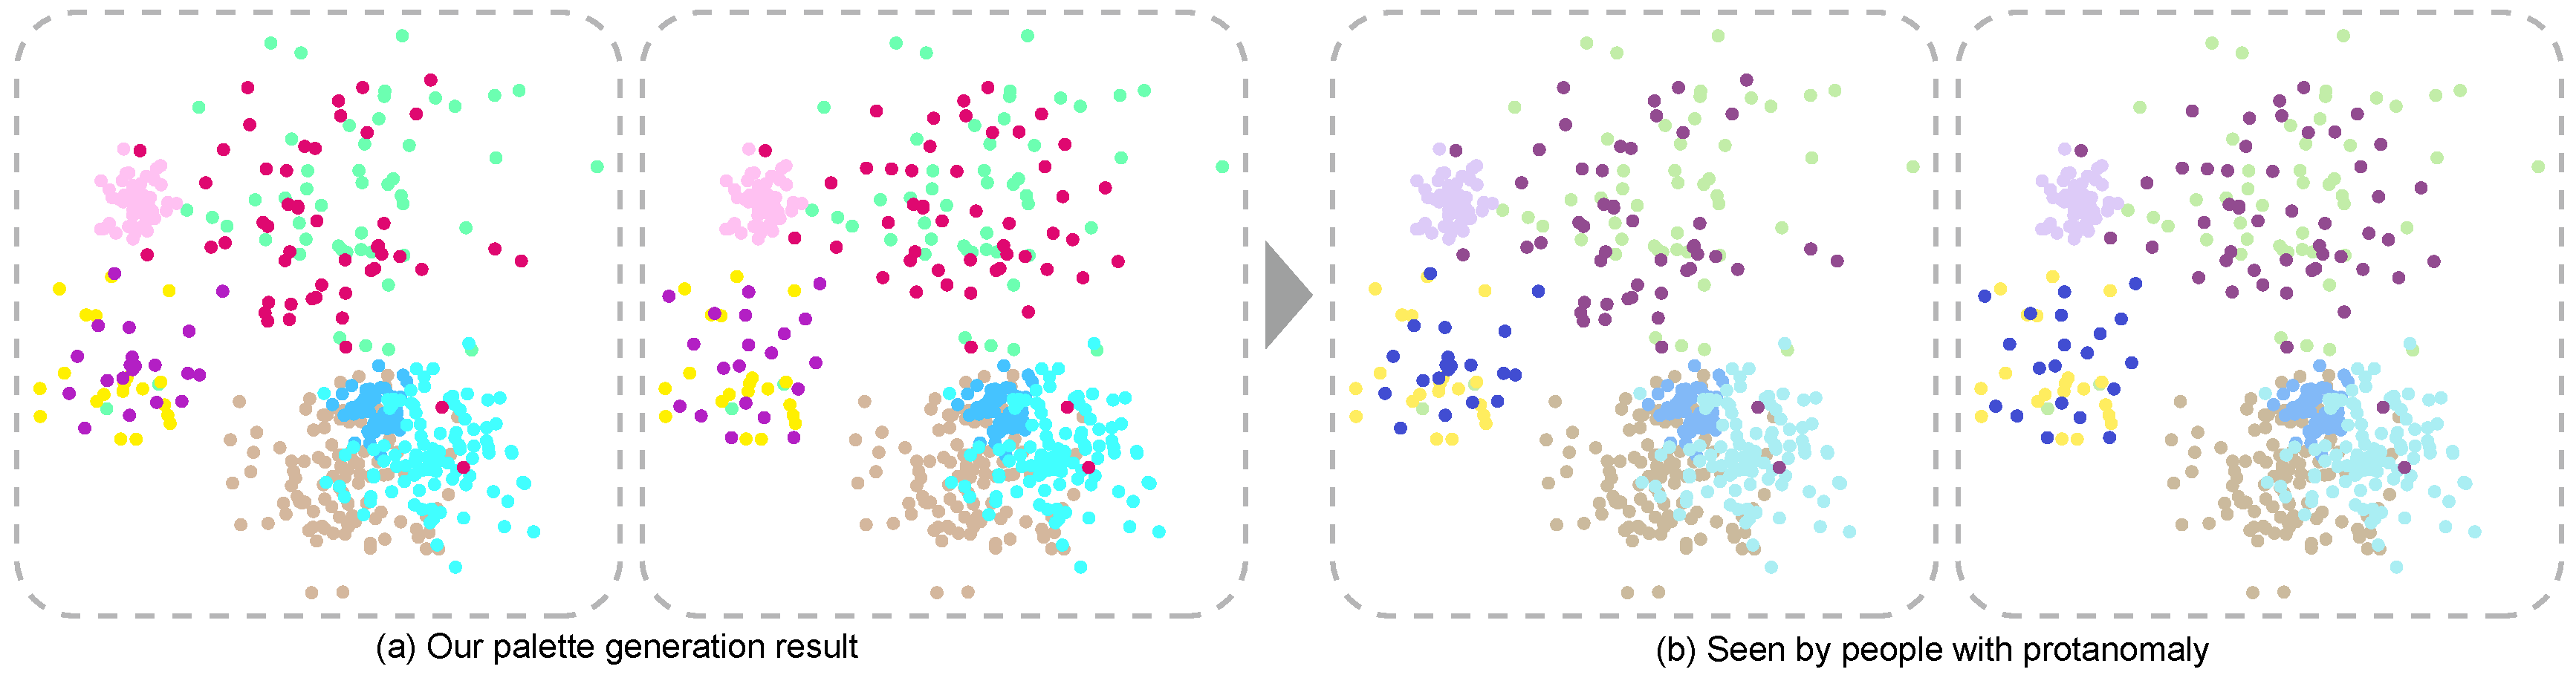
\includegraphics[width=0.96\linewidth]{figures/blindness.pdf}
\caption{Exploring the ability of our system to generate palettes for both people with normal vision and color blindness. (a) The automatic generated palette makes the two importance classes with large saliency while maintain good separability between other classes. (b) Simulated results for people with protanomaly. We can see our results maintain a good performance for color vision deficiency.}
\vspace*{-3mm}
\label{fig:blindness}
\end{figure}


\section {Evaluation}
\label{sec:results}

We evaluated the effectiveness of our method on supporting juxtaposed visual comparisons and the discriminability for reading scatterplots. % by applying it to scatterplots, as scatterplots are commonly used  for such comparisons.
We conducted two online controlled experiments through Amazon Mechanical Turk (AMT) with 217 participants in total, to evaluate how well our method can support people in \emph{observing changes} and \emph{visual separability} for multiple categorical scatterplots:
\begin{enumerate}
%\vspace{-3mm}
\item [(i)] \emph{Spotting the difference task}. To evaluate how well our method can support people in \emph{observing changes} for juxtaposed categorical scatterplots;
%\vspace{-3mm}
\item [(ii)] \emph{Counting class number task}. To evaluate whether our method can support the \emph{visual separability} of classes in each individual scatterplot, which is considered fundamental to juxtaposed comparison.
%%\vspace{-3mm}
%\item [(iii)] an eye tracking study to initially explore if our method helps people \emph{alleviate eye movement distance} when performing  juxtaposed comparison tasks.
%\vspace{-3mm}
%\item [(iv)] performing two case studies to show the usability of our methods for scatterplot matrix and time series data.
\end{enumerate}
%we use synthetic data for the first three studies while use real world data for the case study.

\vspace{.3em}
\noindent{\textbf{Independent Variables.}} In each of our studies, we investigated three independent variables: colorization method, change magnitude and change type.

\emph{Colorization method}: We used six different ways to colorize scatterplots, including four benchmark methods (\emph{Random Assignment}, \emph{Optimized Assignment}, \emph{Alpha Blending} and \emph{Palettailor}) and two experimental methods based on our approach (\emph{C3-Palette Assignment}, \emph{C3-Palette Generation}):
\begin{itemize}

     \item C1: \emph{Random Assignment} is randomly selecting and assigning colors from Tableau-20 palette to the classes.

     \item C2: \emph{Optimized Assignment} uses the optimized assignment approach~\cite{Wang2018} for one of the two scatterplots with an input of Tableau-20 color palette.

     \item C3: \emph{Alpha Blending} is achieved by setting the alpha of each unchanged class to $0.5$ while the changed classes remain to $1.0$ based on \emph{Optimized Assignment} result. We choose $0.5$ since the results also used in the discrimination task.
     \item C4: \emph{Palettailor} uses the method proposed by Lu et.al~\cite{Lu21} for single scatterplot palette generation. The palette is generated for one of the two scatterplots with the default settings.
     \item C5: \emph{C3-Palette Assignment} uses the color assignment optimization solution(Eq.~\ref{eq:cosaliency}) based on Tableau-20.
     \item C6: \emph{C3-Palette Generation} uses the unified color generation and assignment optimization method, and produced the results with the default settings($\omega_0=1.0$, $\omega_1=1.0$ and $\omega_2=1.0$).
\end{itemize}
Our approach are all using the default parameters $\lambda=0.4$ and $\kappa=0$.

\emph{Change magnitude} and \emph{Change type}: While the colorization method is the primary independent variable to be investigated, we are also interested in how the effect of different methods would vary based on the level of change between the two scatterplots and the different change type of classes. Thus we first define two types of changes that a class would have across multiple scatterplots: \emph{point number} and \emph{point position}. Then for each change type, we define three levels of change magnitude calculated using Eq.~\ref{eq:cm}: \emph{small}, \emph{medium}, and \emph{large}. (See the next paragraph for the detailed calculation.)

\vspace{.3em}
\noindent{\textbf{Scatterplot Dataset Generation.}}
The paired scatterplot datasets used in our studies were generated as follows.
First, we designed a set of multi-class scatterplots, each containing $8$ classes. Each class was generated using Gaussian random sampling and placed randomly in a $600 \times 600$ area.
Similar to~\cite{Lu21}, these classes belong to one of the four settings of varying size and density: small \& dense ($n=50, \sigma=20$), small \& sparse ($n=20, \sigma=50$),  large \& dense ($n=100, \sigma=50$), and large \& sparse (($n=50, \sigma=100$).

Then, for each scatterplot generated above, we produced its paired scatterplot by randomly choosing one or more classes and changing the positions or number of their data points.
%We focused on two common change types: \emph{point number} and \emph{point position}.
To systematically compute the changes, we defined two variables: \emph{change ratio} and \emph{number of changed classes}.
\emph{Change ratio} defines how large the change of a type is, ranging from 0 to 1; and {number of changed classes} defines the number of classes that are changed, ranging from 1 to 3 (to add
different levels of difficulty). We summarize our basic idea of data generation for each change type as below.
\begin{itemize}

     \item \emph{Point number}: For each class in the original scatterplot,  we calculated the new point number by multiplying the original number by ($1 \pm$ \emph{change ratio}). An addition means to increase the point number, which was implemented by generating the new points with the same distribution as the original class. Subtraction was achieved by randomly deleting data points from the original class.

     \item \emph{Point position}: Point position contains many types, such as class center position change and shape change. In our experiment, we use the two different position changes mentioned above. For center position change, the center of a class can be moved in a certain \emph{direction} with a specific \emph{distance}. We moved the center towards a random direction by a distance calculated by multiplying a maximal change distance ($400$ by default) by the \emph{change ratio}. For shape change, we define the shape of a class as the bounding box of its data points. We simulated a shape change of a class by modifying the density parameter of its Gaussian distribution to the opposite direction. For example, a small \& dense class ($n=50, \sigma=20$) would be changed into a small \& sparse ($n=50, \sigma=50$) class. In order to produce a new shape for a class, we first calculate the one-to-one mapping between the newly-generated class and the original class using ~\cite{kuhn1955hungarian} and then linearly interpolated the new point between each two points based on the \emph{change ratio} parameter. We randomly choose one change type when disturbing the class to be changed.
\end{itemize}
For each change type, we produced 300 candidate scatterplot pairs and then calculated the \emph{change magnitude} for each pair, and split all  pairs into three levels: \emph{small},  \emph{medium}, and \emph{large}.
Next, we randomly selected $2$ pairs from each change magnitude level for each change type and each number of changed classes. Thus in total we used $36$ paired scatterplot in each of the two studies. The detailed dataset is showed in Table.~\ref{tab:latinsquare}

\begin{table}[ht]
     \renewcommand\arraystretch{1}
     \centering
     \caption{Grouping of Datasets: $36$ datasets $\times$ $6$ conditions. C: condition; G: participant group; Position Small 1: point position change with small change magnitude for 1 changed class.}
     \label{tab:latinsquare}
     \begin{tabular}{lcccccccc}
     \hline
      & C1 & C2 & C3  & C4 & C5 & C6 \\

     \hline
     Dataset 1: Position Small 1 & \textbf{G1} & G2 & G3  & G4 & G5 & G6 \\
     Dataset 2: Position Small 1 & G6 & \textbf{G1} & G2 & G3  & G4 & G5 \\
     Dataset 3: Position Small 2 & G5  & G6 & \textbf{G1} & G2 & G3 & G4 \\
     Dataset 4: Position Small 2 & G4 & G5  & G6 & \textbf{G1} & G2 & G3 \\
     Dataset 5: Position Small 3 & G3 & G4 & G5  & G6 & \textbf{G1} & G2 \\
     Dataset 6: Position Small 3 & G2 & G3 & G4  & G5 & G6 & \textbf{G1} \\
     Dataset 7: Position Medium 1 & \textbf{G1} & G2 & G3  & G4 & G5 & G6 \\
     Dataset 8: Position Medium 1 & G6 & \textbf{G1} & G2 & G3  & G4 & G5 \\
     ... & & & & & & &\\
     Dataset 35: Number Large 3 & G3 & G4 & G5  & G6 & \textbf{G1} & G2 \\
     Dataset 36: Number Large 3 & G2 & G3  & G4 & G5 & G6 & \textbf{G1}  \\

     \hline
     \end{tabular}
     \end{table}
%
%\subsection{Numeric Study}
%\label{subsec:quantitystudy}
%To evaluate whether our approach can fundamentally support the visual separability of the classes in each scatterplot, we conducted a numeric study using the \emph{class visibility metric} proposed by Kim et al.~\cite{lee2013perceptually}. We calculated each scatterplot in every pair, and used the average value as the final score of the pair. We then compared the scores across different colorization methods.
%
%%\vspace{.3em}
%%\noindent{\textbf{Results.}}
%
%\begin{figure}[h]
%\centering
%\includegraphics[width=0.9\linewidth]{figures/classVisibility.pdf}
%\caption{Average class visibility score of the 36 synthetic scatterplot pairs of each color mapping scheme.}
%\vspace*{-3mm}
%\label{fig:classVisibility}
%\end{figure}
%
%As shown in Fig.~\ref{fig:classVisibility}, \emph{Ours Generation} has the highest score on average. \emph{Ours Tableau-10} is sometimes higher than \emph{Random Tableau-10}. The two conditions based on the Tableau-20 palette have the lowest scores, and \emph{Ours Tableau-20} appears to be slightly lower than \emph{Random Tableau-20}. This might be caused by the palette used in these conditions. Since Tableau-20 consists of both saturated and de-saturated colors, \emph{Ours Tableau-20} tends to select several de-saturated colors for the classes that change less in order to make strongly changed classes more salient. Yet that might diminish the visual separability of the classes.

\subsection{Experiment 1: Spotting the Difference}
\label{subsec:onlinestudy1}

To evaluate how well our approach can assist observing changes between juxtaposed categorical scatterplots, we conduct an online ``spot-the-difference'' experiment through Amazon Mechanical Turk (AMT) with 136 participants.
%We show participants a set of paired multi-class scatterplots, and ask them to find a known number of classes that have been changed within $60$ seconds.  Error rate and consuming time are recorded for analysis.

\vspace{.3em}
\noindent{\textbf{Hypotheses.}} We hypothesized that our approach would generally be more effective than the benchmark methods on the juxtaposed comparison tasks, and that this effect would vary based on \emph{change magnitude} or \emph{change type}.
%In this experiment, our major goal is to investigate if our co-saliency based color design formulation would affect the performance of observing changes between multiple datasets.
\begin{itemize}[noitemsep]
\setlength{\itemsep}{5pt}
    \item[\textbf{H1.}] Our color generation method (\emph{C3-Palette Generation}) outperforms the benchmark conditions (\emph{Random Assignment}, \emph{Optimized Assignment}, \emph{Alpha Blending} and \emph{Palettailor}) on the task performance.

    \item [\textbf{H2.}] Our color assignment method (\emph{C3-Palette Assignment}) using a color palette with a large range of brightness and saturation (\emph{Tableau-20}) outperforms the benchmark conditions (\emph{Random Assignment}, \emph{Optimized Assignment}, \emph{Alpha Blending} and \emph{Palettailor}) on the task performance.

    \item [\textbf{H3.}] Other independent variables(\emph{change type} and \emph{change magnitude}) would also affect user performance on the task performance.

    \item [\textbf{H4.}] There would be an interaction effect between colorization methods and other independent variables(\emph{change type} and \emph{change magnitude}). Specifically, the difference between the effect of our methods (\emph{C3-Palette Generation} and \emph{C3-Palette Assignment}) and that of the benchmark methods (\emph{Random Assignment}, \emph{Optimized Assignment}, \emph{Alpha Blending} and \emph{Palettailor}) would change based on the different variable.
\end{itemize}

% For content we can refer to:
% \url{http://www.yunhaiwang.net/infoVis2020/palettailor/pdf/vis20a-sub1326-i6.pdf}
% \begin{itemize}
%     \item List the assignment methods: ours and the benchmarks.
%     \item Recap the definition of \emph{change magnitude} and \emph{change type}.
% \end{itemize}

\subsubsection{Experimental Design}
%In this experiment, each participant completed a ``spot-the-difference'' task that contains $40$ paired multi-class scatterplots.
%To colorize the paired scatterplots, we adopt the five visualization methods -- three of them are optimized or generated based on our approach (\emph{Ours Tableau-10}, \emph{Ours Tableau-20} and \emph{Ours Generation}), while the other two are random ones  (\emph{Random Tableau-10} and \emph{Random Tableau-20}).
\
\newline
\vspace{.3em}
\noindent{\textbf{Task \& Measures.}}
In this experiment, each participant was asked to perform a \emph{spot-the-difference} task. Inspired by the Spot the Difference game where one needs to compare a pair of similar pictures to detect their differences~\cite{Fukuba2009}, we asked participants to identify all the classes that have been changed in two scatterplots. At the beginning of each trial, the number of changed classes was provided. Each participant was asked to select all the changed classes by clicking the points belonging to these classes in either of the scatterplots.

For each participant, we measured the \emph{time} taken for each trial, and counted the errors ($0/1$) indicating whether the actual changed classes are aligned with the participant's response. Note that if any of the changed classes was mistakenly identified, the trial would be considered as ``wrong'' (1).

While the participant was instructed to do the task ``\emph{as accurately as possible}'', we set a $60$-second time limit for each trial for fear that user might spend too much time on the trial. If the participant could not find all the changed classes during the time limit, they were directed to the next trial. There also will appear a ``\emph{Can't Find it}'' button after $30$ seconds.
This was done since we observed from the pilot study that when participants spent too much time on a single trial, they may decide to quit by selecting a class randomly(which will lead to an incorrect answer) or to spend more time till they get the correct answer or the time limit (which will lead to increasing time spent on the trial). This subject decision would add noise to our measurements. Thus we added a $30$-second time limit, which was informed by our pilot study, where over $85\%$ correct trials were completed within $30$ seconds.

\vspace{.3em}
\noindent{\textbf{Experiment Organization.}} We tested the effects of the $6$ method conditions across $36$ paired multi-class scatterplot datasets using a \emph{between-subject} experiment design. To avoid ordering effects, where the participant would get familiar with a dataset after seeing it several times, each participant was assigned to a group and saw a specific subset of datasets under different conditions. We used a Latin Square grouping (see Table.~\ref{tab:latinsquare}) to organize the trials for each participant. %$Thus, there were $6$ participant groups and each of them had $40$ trials in total. See the supplementary material for more details.

In addition, some participants might apply a ``shortcut'' strategy when seeing a class that is obviously more salient than the others, especially under the \emph{C3-Palette Assignment} and \emph{C3-Palette Generation} conditions. Thus, for quality control, we added $4$ sentinels which were very simple trials with only one changed class and a large change magnitude, and we assigned a de-saturated color to the changed class that made it less salient. We add these 4 distractor trials to each group to identify whether the participants is doing the task seriously and reject the results with more than two wrong trials.
%especially to avoid preferences of \emph{Our Generation} method.
%Only answers with a over $50\%$ accuracy were accepted.

Finally, there were $6$ participant groups and each of them had $40$ trials in total. To further avoid learning effects between trials, we randomly shuffled the display orders of all scatterplot pairs, and randomly placed the two scatterplots in each pair on the left or right side.

\begin{table}[ht]
\renewcommand\arraystretch{1}
\centering
\caption{Participants details for each task.}
\label{tab:participantDetail}
\begin{tabular}{|c|c|c|c|c|}
\hline
\multirow{2}{*}{\textbf{Task \& Group}} & \multicolumn{2}{c|}{Spotting the Difference} & \multicolumn{2}{c|}{Counting class number} \\
\cline{2-5}
& Pilot(28) & Formal(108) & Pilot(29) & formal(52) \\
\hline
Group 1 & 5 & 18 & 5  & 9 \\
\hline
Group 2 & 5 & 17 & 5  & 8 \\
\hline
Group 3 & 5 & 19 & 4  & 8 \\
\hline
Group 4 & 3 & 17 & 5  & 9 \\
\hline
Group 5 & 5 & 19 & 5  & 9 \\
\hline
Group 6 & 5 & 18 & 5  & 9 \\
\hline
\end{tabular}
\end{table}

\begin{figure*}[t]
\centering
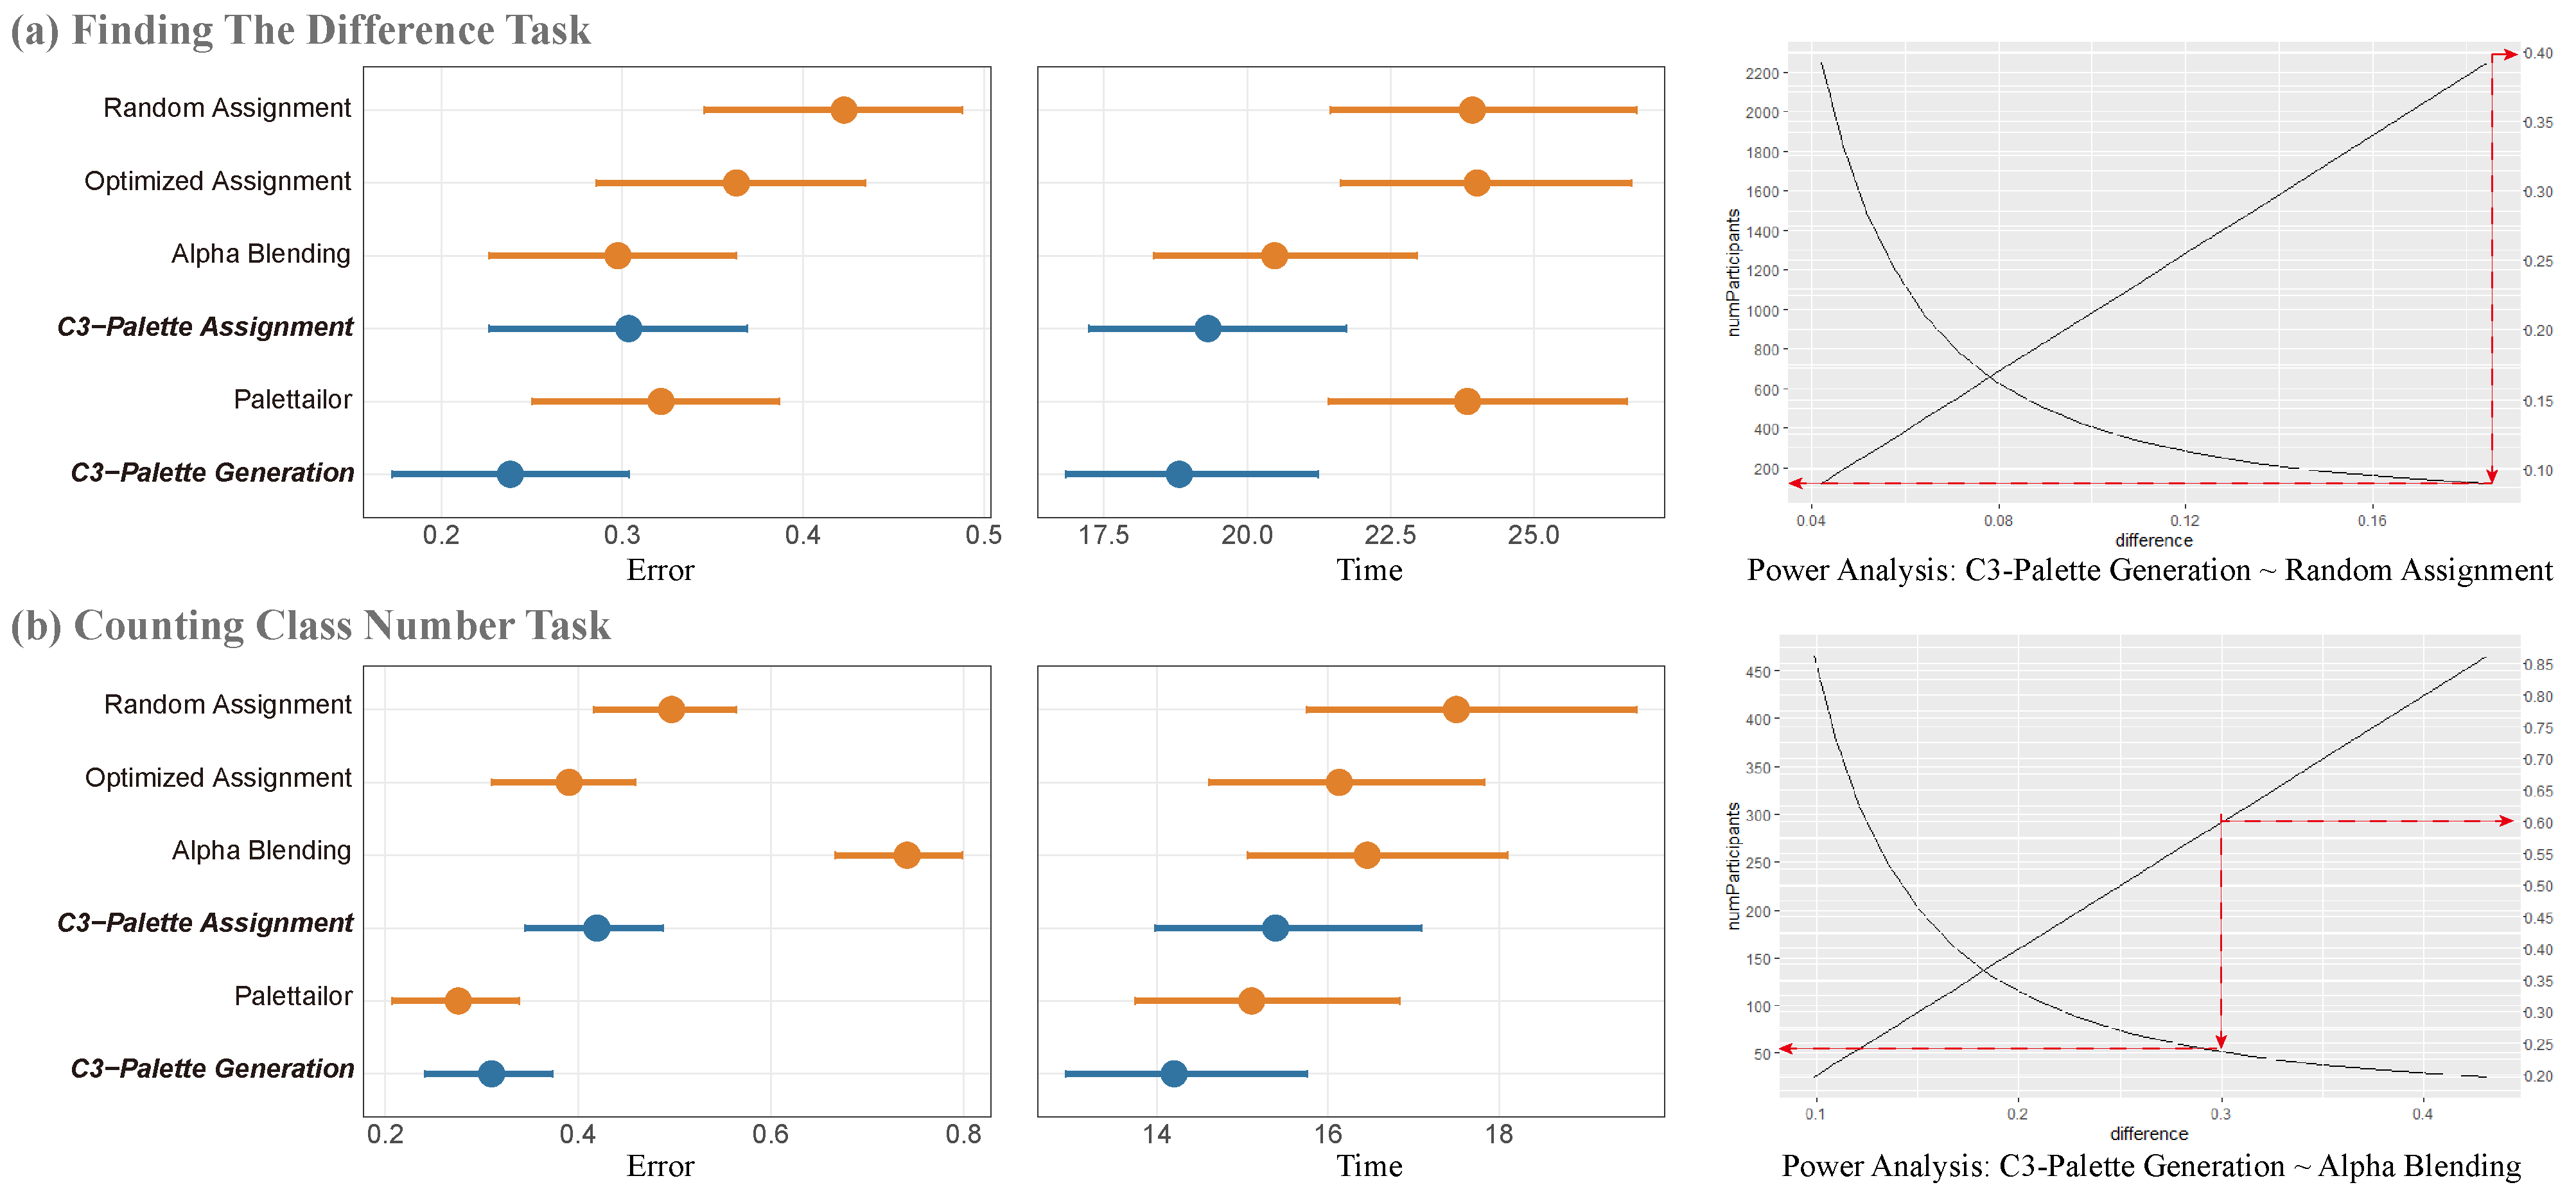
\includegraphics[width=1\linewidth]{figures/user-result-pilot.pdf}
\caption{Confidence interval plots and power analysis for the two pilot studies.
}
\vspace*{-3mm}
\label{fig:pilotResults}
\end{figure*}

\vspace{.3em}
\noindent{\textbf{Pilot Study \& Power Analysis.}}
We conducted a pilot study involving 28 participants to check the experimental setup and determine the parameters, such as the time limit for a trial. The results are shown in Fig.~\ref{fig:pilotResults}(a).
Harnessing by the pilot study, we also obtained our expected effect sizes, which were in further fed into a power analysis. With an effect size Cohen's $d$ of $0.4$, alpha level of $0.05$ and beta level of $0.8$, the power analysis suggested a minimum number of $100$ participants for the spot-the-difference task. %See the supplementary material for more details.


\vspace{.3em}
\noindent{\textbf{Participants.}}
We recruited $108$ participants(as shown in Table.~\ref{tab:participantDetail}) for the experiment on Amazon Mechanical Turk.
According to the completion time in the pilot study, we paid each participant \$$1.5$ for the task based on the US minimum hourly wage.
No participant claimed color vision deficiency on their informed consent.

\vspace{.3em}
\noindent{\textbf{Procedure.}}
Each participant went through the following steps in our experiment: (i) viewing a user guide of the task and completing three training trials; (ii) completing each trial as accurately as possible; (iii) providing demographic information.

\begin{figure*}[t]
\centering
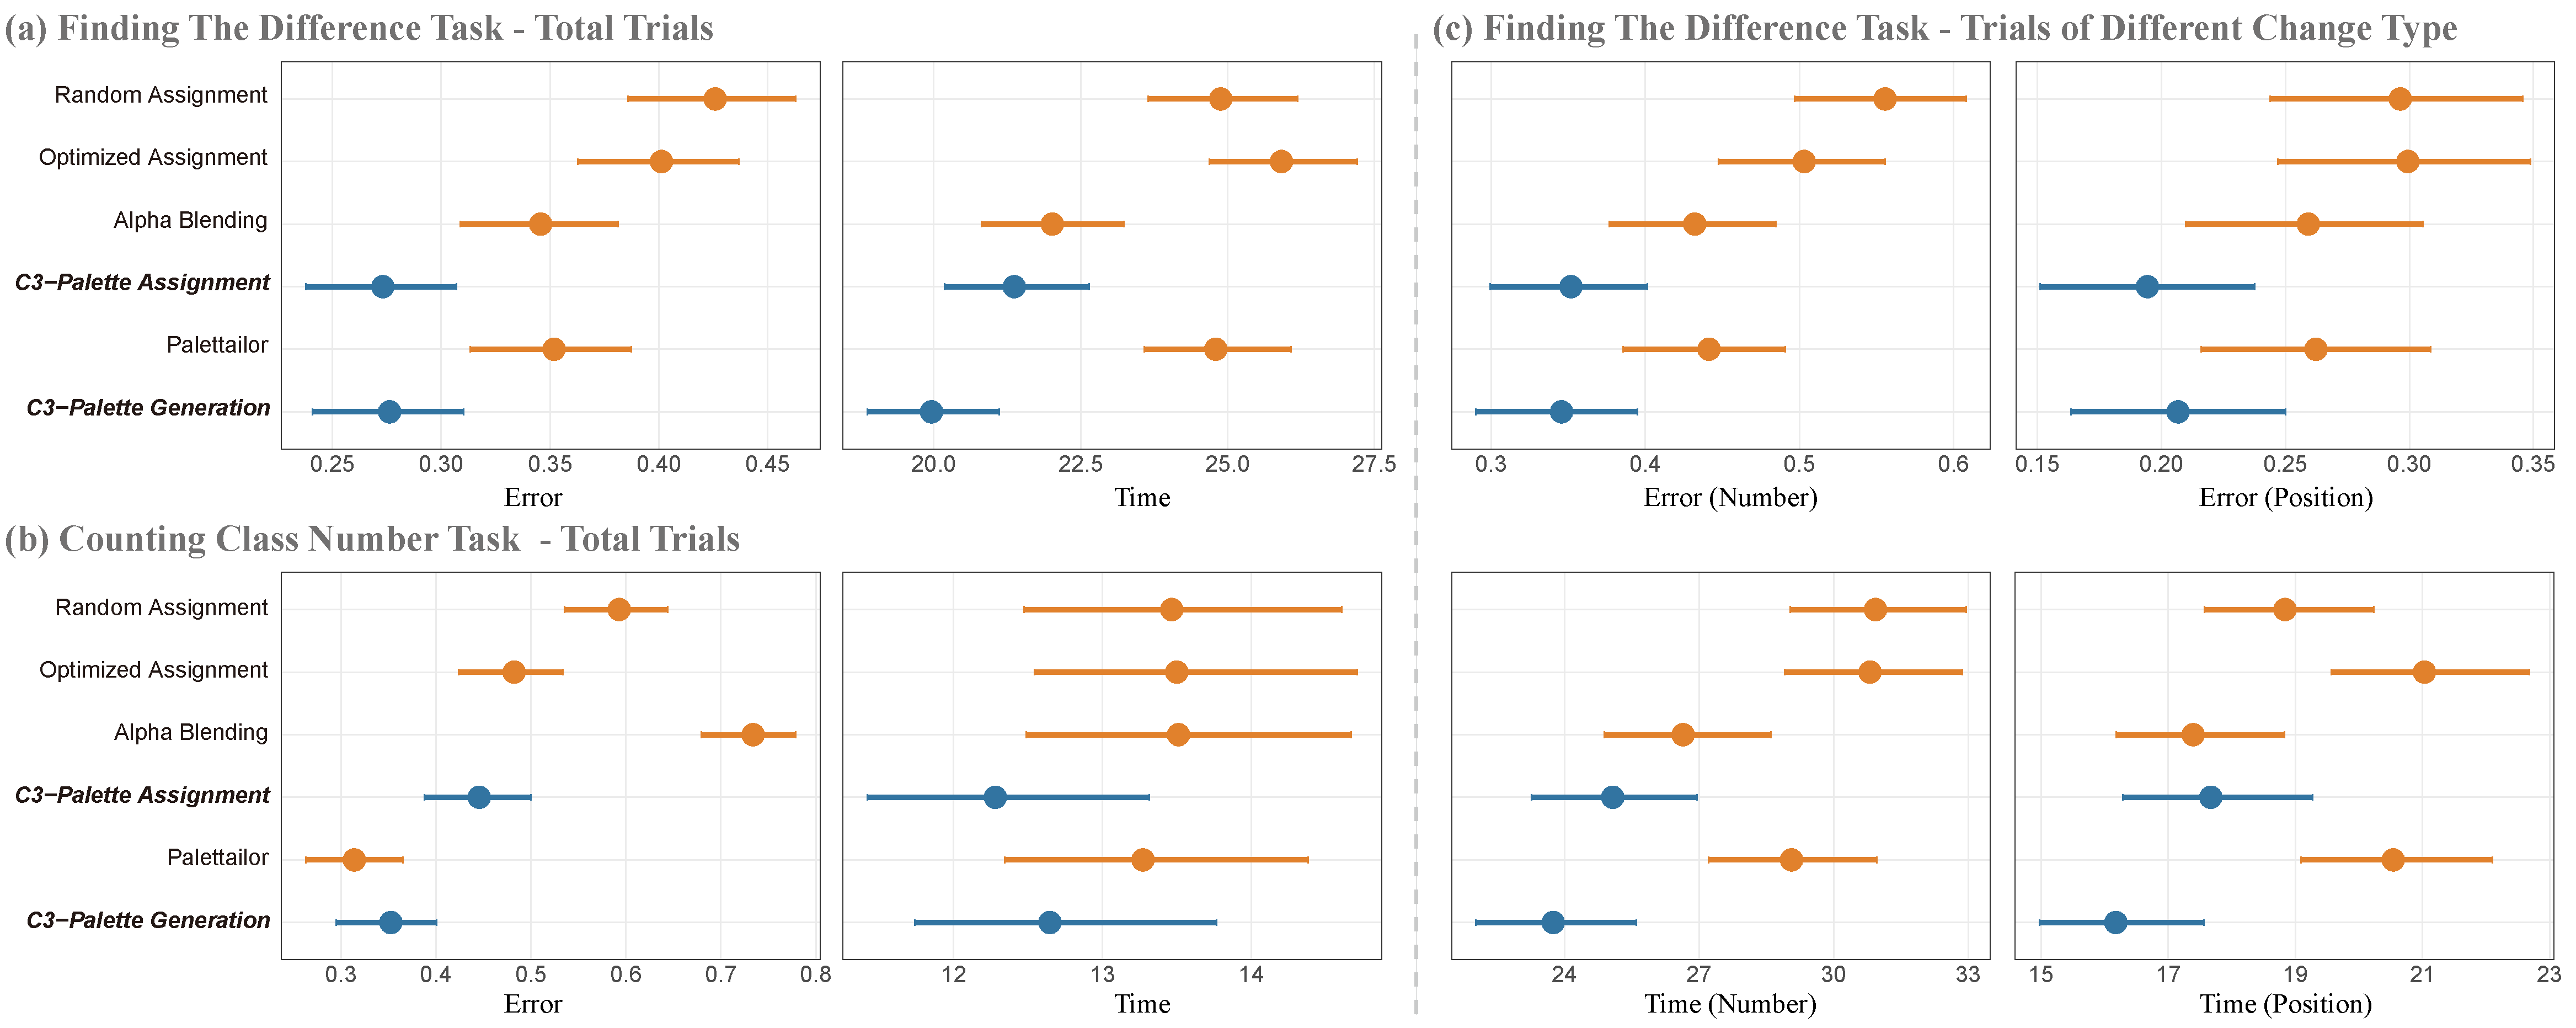
\includegraphics[width=1\linewidth]{figures/user-result-formal.pdf}
\caption{Confidence interval plots and statistical tables for the two online controlled experiments. Error bars represent $95\%$ confidence intervals. Each table shows the statistical test results of C3-Palette Generation condition with other conditions, including the mean with $95\%$ confidence interval ($\mu\sim$95\%CI), the W-value and p-value from the Mann-Whitney test, and the effect size ($d\sim$95\%CI).
}
\vspace*{-3mm}
\label{fig:userResults}
\end{figure*}

\subsubsection{Results}
\
\newline
Following previous studies, we analyzed the results using 95\% confidence intervals, and also conducted Mann-Whitney tests to compare the differences between conditions. The non-parametric test was used due to observations of non-normally distributed data from our pilot study. In addition, we computed the effect size using \emph{Cohen's d}, i.e., the difference in means of the conditions divided by the pooled standard deviation. We used ANOVA to examine the interaction effect between variables.


Results of the online experiment are shown in Fig.\ref{fig:userResults} (a).
First, we found that our approach(\emph{C3-Palette Assignment} and \emph{C3-Palette Generation}) leads to a significantly lower error rate than all benchmark conditions. For consuming time, \emph{C3-Palette Generation} has significantly less time (\emph{$p = 0.003$}) than \emph{Alpha Blending} condition while \emph{C3-Palette Assignment} has no significant difference (\emph{$p = 0.095$}), and our approach has significantly less time than all other benchmark conditions(\emph{$p < 0.001$}). The result indicates that our palette generation method(\emph{C3-Palette Generation}) has a better performance than benchmark conditions in the ``spot-the-difference'' task (\textbf{H1} confirmed). As for color palette with a larger range of brightness and saturation, our approach(\emph{C3-Palette Assignment}) is better than most conditions and is at least comparable to \emph{Alpha Blending} condition(\textbf{H2} confirmed).


%Second, we compared our approach to other conditions based on two different change types(\emph{Point Number Change} and \emph{Point Position Change}).
%For \emph{Point Number Change}, as shown in the top row of  Fig.\ref{fig:userResults} (c), our approach(\emph{C3-Palette Assignment} and \emph{C3-Palette Generation}) leads to a significantly lower error rate than all benchmark conditions, including \emph{Random Assignment} and \emph{Optimized Assignment}(\emph{$p < 0.001$}), \emph{Alpha Blending} and \emph{Palettailor}(\emph{$p < 0.05$}). \emph{C3-Palette Generation} condition has a better performance on consuming time than all other benchmark conditions, while \emph{C3-Palette Assignment} is just comparable to \emph{Alpha Blending} condition.
%For \emph{Point Position Change}, we observed that our approach has significant lower error rate than \emph{Random Assignment} and \emph{Optimized Assignment}(\emph{$p < 0.01$}), while there's no significant difference with \emph{Alpha Blending} and \emph{Palettailor}. \emph{C3-Palette Generation}) leads to a significantly lower consuming time than all benchmark conditions(\emph{$p < 0.001$}) except \emph{Alpha Blending}(\emph{$p = 0.044$})(\textbf{H3} confirmed).
Second, we compared error and time with regard to different change magnitudes, and found that smaller magnitude leads to larger error rate and consuming time (as shown in Fig.\ref{fig:userResultsVar} (a) left). This indicates that there exists an significant interaction effect between \emph{change magnitude} and performance, i.e., \emph{change magnitude} would affect user performance. We did the same test to \emph{change type}, the results show that \emph{point number change} is much more difficult than \emph{point position change}(\textbf{H3} confirmed).


Finally, we did not find significant interaction effect between \emph{colorization methods} and \emph{change magnitude} or \emph{change type}, meaning that the effect of our method is not necessarily influenced by the magnitude of change between the two scatterplots or the different change type of classes (\textbf{H4} not confirmed).

\begin{figure*}[h]
\centering
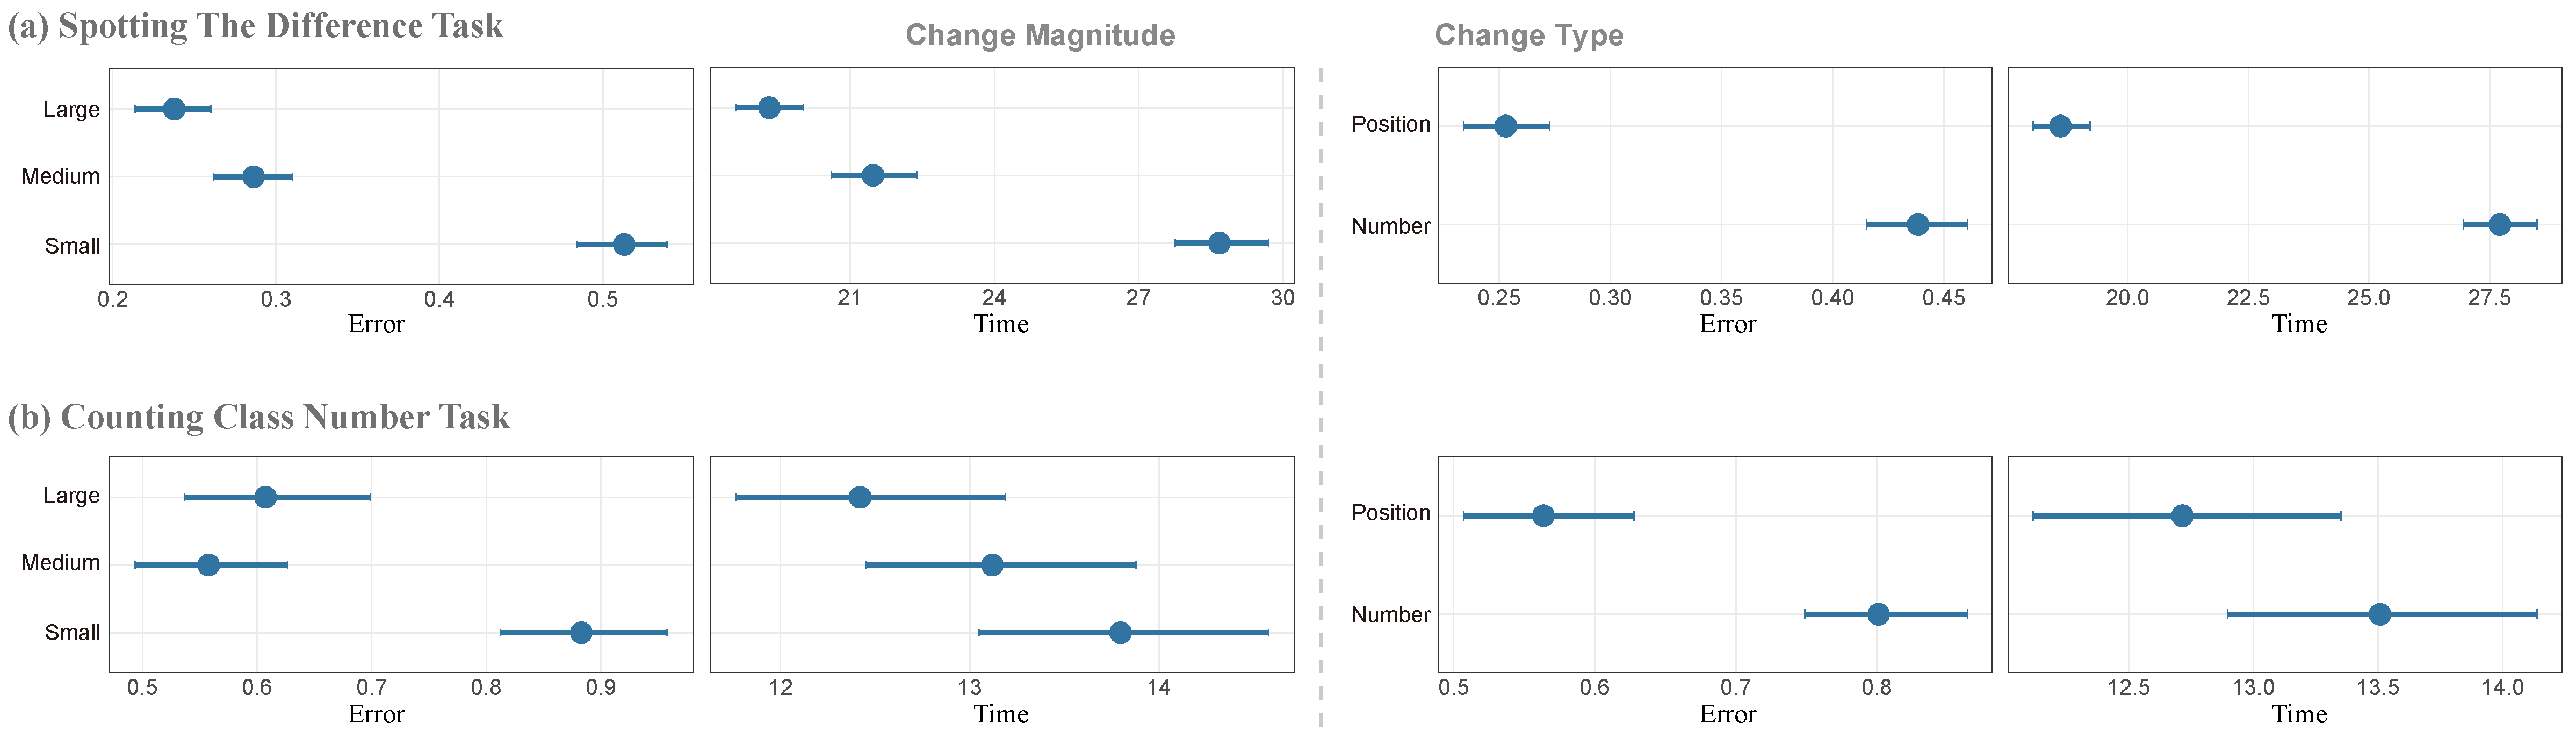
\includegraphics[width=1\linewidth]{figures/user-result-formal-variables.pdf}
\caption{Confidence interval plots for the two online controlled experiments. (left) Plots for \emph{change magnitude} based on error and time; (right) plots for \emph{change type} based on error and time.
}
\vspace*{-3mm}
\label{fig:userResultsVar}
\end{figure*}

\subsection{Experiment 2: Counting Class Number}
\label{subsec:onlinestudy2}
To evaluate whether our approach can fundamentally support the visual separability of the classes in each scatterplot, we conduct an online ``counting class number'' experiment through Amazon Mechanical Turk (AMT) with 81 participants. The experimental design was similar to the first study, but we set up with different task during the experiment.
We expected to see different patterns of the discriminability across different conditions. Specifically, our methods would lead to a shorter error and time than \emph{Random Assignment} and \emph{Alpha Blending} conditions.

\vspace{.3em}
\noindent{\textbf{Hypotheses.}} We hypothesized that our approach would generally be more effective than the benchmark methods on the discrimination tasks, and that this effect would not vary based on \emph{change magnitude} or \emph{change type}.
\begin{itemize}[noitemsep]
\setlength{\itemsep}{5pt}
    \item[\textbf{H1.}] Our color generation method (\emph{C3-Palette Generation}) outperforms the benchmark conditions (\emph{Random Assignment}, \emph{Optimized Assignment}, \emph{Alpha Blending}) and our assignment method(\emph{C3-Palette Assignment}), while is comparable to  \emph{Palettailor} on the task performance.

    \item [\textbf{H2.}] Our color assignment method (\emph{C3-Palette Assignment}) based on \emph{Tableau-20} outperforms the benchmark conditions (\emph{Random Assignment}, \emph{Alpha Blending}), while is comparable to \emph{Optimized Assignment} condition on the task performance.

    \item [\textbf{H3.}] Other independent variables(\emph{change magnitude} and \emph{change type}) would have no effect on discrimination task between different conditions.

    \item [\textbf{H4.}] There would be no interaction effect between colorization methods and other independent variables(\emph{change type} and \emph{change magnitude}).
\end{itemize}
\subsubsection{Experimental Design}
\
\newline
\vspace{.3em}
\noindent{\textbf{Task \& Measures. }}
Following previous methodologies~\cite{Wang2018, Lu21}, each participant was asked to perform a \emph{counting class number} task.  We asked participants to identify how many classes(colors) are there in the given two scatterplots and then choose an answer among several options below the two scatterplots. We recorded the participant's answer and response time for each trial, and counted the \emph{error}  by calculating the differences between the participant's answer and the actual number of classes(each scatterplot has $8$ classes in our experiment). %is $1$ if the participant's response not equal to the actual class number, else $0$.


\vspace{.3em}
\noindent{\textbf{Pilot Study \& Power Analysis.}}
This setting is similar to Experiment 1. We invited $29$ participants to do the pilot study and the results were in further fed into a power analysis. With an effect size Cohen's $d$ of $0.6$, the power analysis suggested a minimum number of $50$ participants for the discriminability task. See the supplementary material for more details.

\vspace{.3em}
\noindent{\textbf{Participants.}}
We finally recruited $52$ participants(as shown in Table.~\ref{tab:participantDetail}) for the experiment on Amazon Mechanical Turk.
According to the completion time in the pilot study, we paid each participant \$$1.5$ for the task based on the US minimum hourly wage.
No participant claimed color vision deficiency on their informed consent.

\subsubsection{Results}
\
\newline
Results of this visual separability experiment are shown in Fig.\ref{fig:userResults} (b).
Through this study we found that first \emph{C3-Palette Generation} is comparable to \emph{Palettailor} while leads to a significantly lower error rate(\emph{$p<=0.001$}) than all other benchmark conditions. Specifically, \emph{C3-Palette Generation} has a significantly lower error rate(\emph{$p=0.002$}) than \emph{C3-Palette Assignment}(\textbf{H1} confirmed).
Second, \emph{C3-Palette Assignment} has higher performance than the benchmark conditions (\emph{Random Assignment}, \emph{Alpha Blending}) and is comparable to \emph{Optimized Assignment}(\textbf{H2} confirmed).
For other independent variables, as shown in Fig.\ref{fig:userResultsVar} (b), we found that there existed a significant difference between \emph{Small change magnitude} and \emph{Medium} and \emph{Large}. \emph{Point position change} has a much lower error rate than \emph{point number change}. And their time has both a tendency to gradually increase. This indicates that \emph{change magnitude} and \emph{change type} might have an effect on discrimination task between different conditions (\textbf{H3} not confirmed).
Finally, we did not find significant interaction effect between \emph{colorization methods} and \emph{change magnitude} or \emph{change type}, meaning that the effect of different methods for visual discriminability is not
necessarily influenced by the magnitude of change between the two scatterplots or the different change type of classes (\textbf{H4} confirmed).
\vspace{.3em}
\subsection{Discussion}
In summary, we evaluated the effectiveness of our approach against the benchmark conditions through two online studies.
We found that first, our methods outperform the benchmark methods on juxtaposed comparison tasks, and their effects are not necessarily influenced by the change magnitude of the two scatterplots or the change type of each class.
The performance of \emph{Optimized Assignment} is comparable to \emph{Random Assignment}, this is reasonable, since \emph{Optimized Assignment} mainly cares about the visual separability of different classes, thus it might assign the less salient color to the changed class while \emph{Random Assignment} would assign salient color even though the whole separability of the scatterplot is not very good. This also provides an explanation for \emph{Alpha Blending} which is based on the result of \emph{Optimized Assignment}.
Second, our experimental methods (\emph{C3-Palette Generation} and \emph{C3-Palette Assignment}) generally support the fundamental visual separability of the classes. It is worth noting that the error rate of \emph{C3-Palette Generation} is comparable to \emph{Palettailor} which is the start-of-the-art palette generation method for visual discriminability, while \emph{C3-Palette Assignment} is comparable to \emph{Optimized Assignment} which is the start-of-the-art palette assignment method for visual discriminability. This indicates that our approach maintains the class distinction of the scatterplot while enhances the class saliency to help observe changes between different scatterplots.
Third, we found that \emph{change magnitude} and \emph{change type} influence the performance of the \emph{counting class number} task. The potential explanation is that large change between scatterplots will attract participants' attention, thus make it easy to distinct different classes. This is also reasonable for \emph{change type} since point position change is easier to distinguish than point number change.
It's obvious that \emph{Alpha Blending} has a much lower error rate than other methods for discrimination task. As one of the participants said, ``The ones that were harder were ones that had colors that when they overlapped would change color. It made it hard to tell if it was the same color or if it was a new color. When the colors were uniform and all the same opacity, it was much easier.'' \emph{Alpha Blending} condition changes the opacity of unchanged classes to make the unchanged classes more distinct, but this will generate new color from color blending, so as to make it hard to distinct colors.

Some limitations exist in our evaluation.
First, our experiment mainly focuses on error rate and time comsuming, while other measurements are not explored, such as click order of the changed classes and time consuming for each click. These might reflect some interesting results for different \emph{cluster type}.
Second, our experiment focuses on identifying the differences between two scatterplots, which is a simplified situation, since in real-world cases often more than two visualizations are compared.
Third, we cannot further analyze the effect of \emph{change type}, given the current study design, though we did observe some trends that for certain types of change, our methods are more effective.
That brings us to a series of more fundamental questions: how can we properly define the types of changes? What is the just noticeable change magnitude for each change type?
Further research is needed to answer these questions so that our approach can be thoroughly evaluated.

\section{Interactive System}


\begin{figure}[ht]
\centering
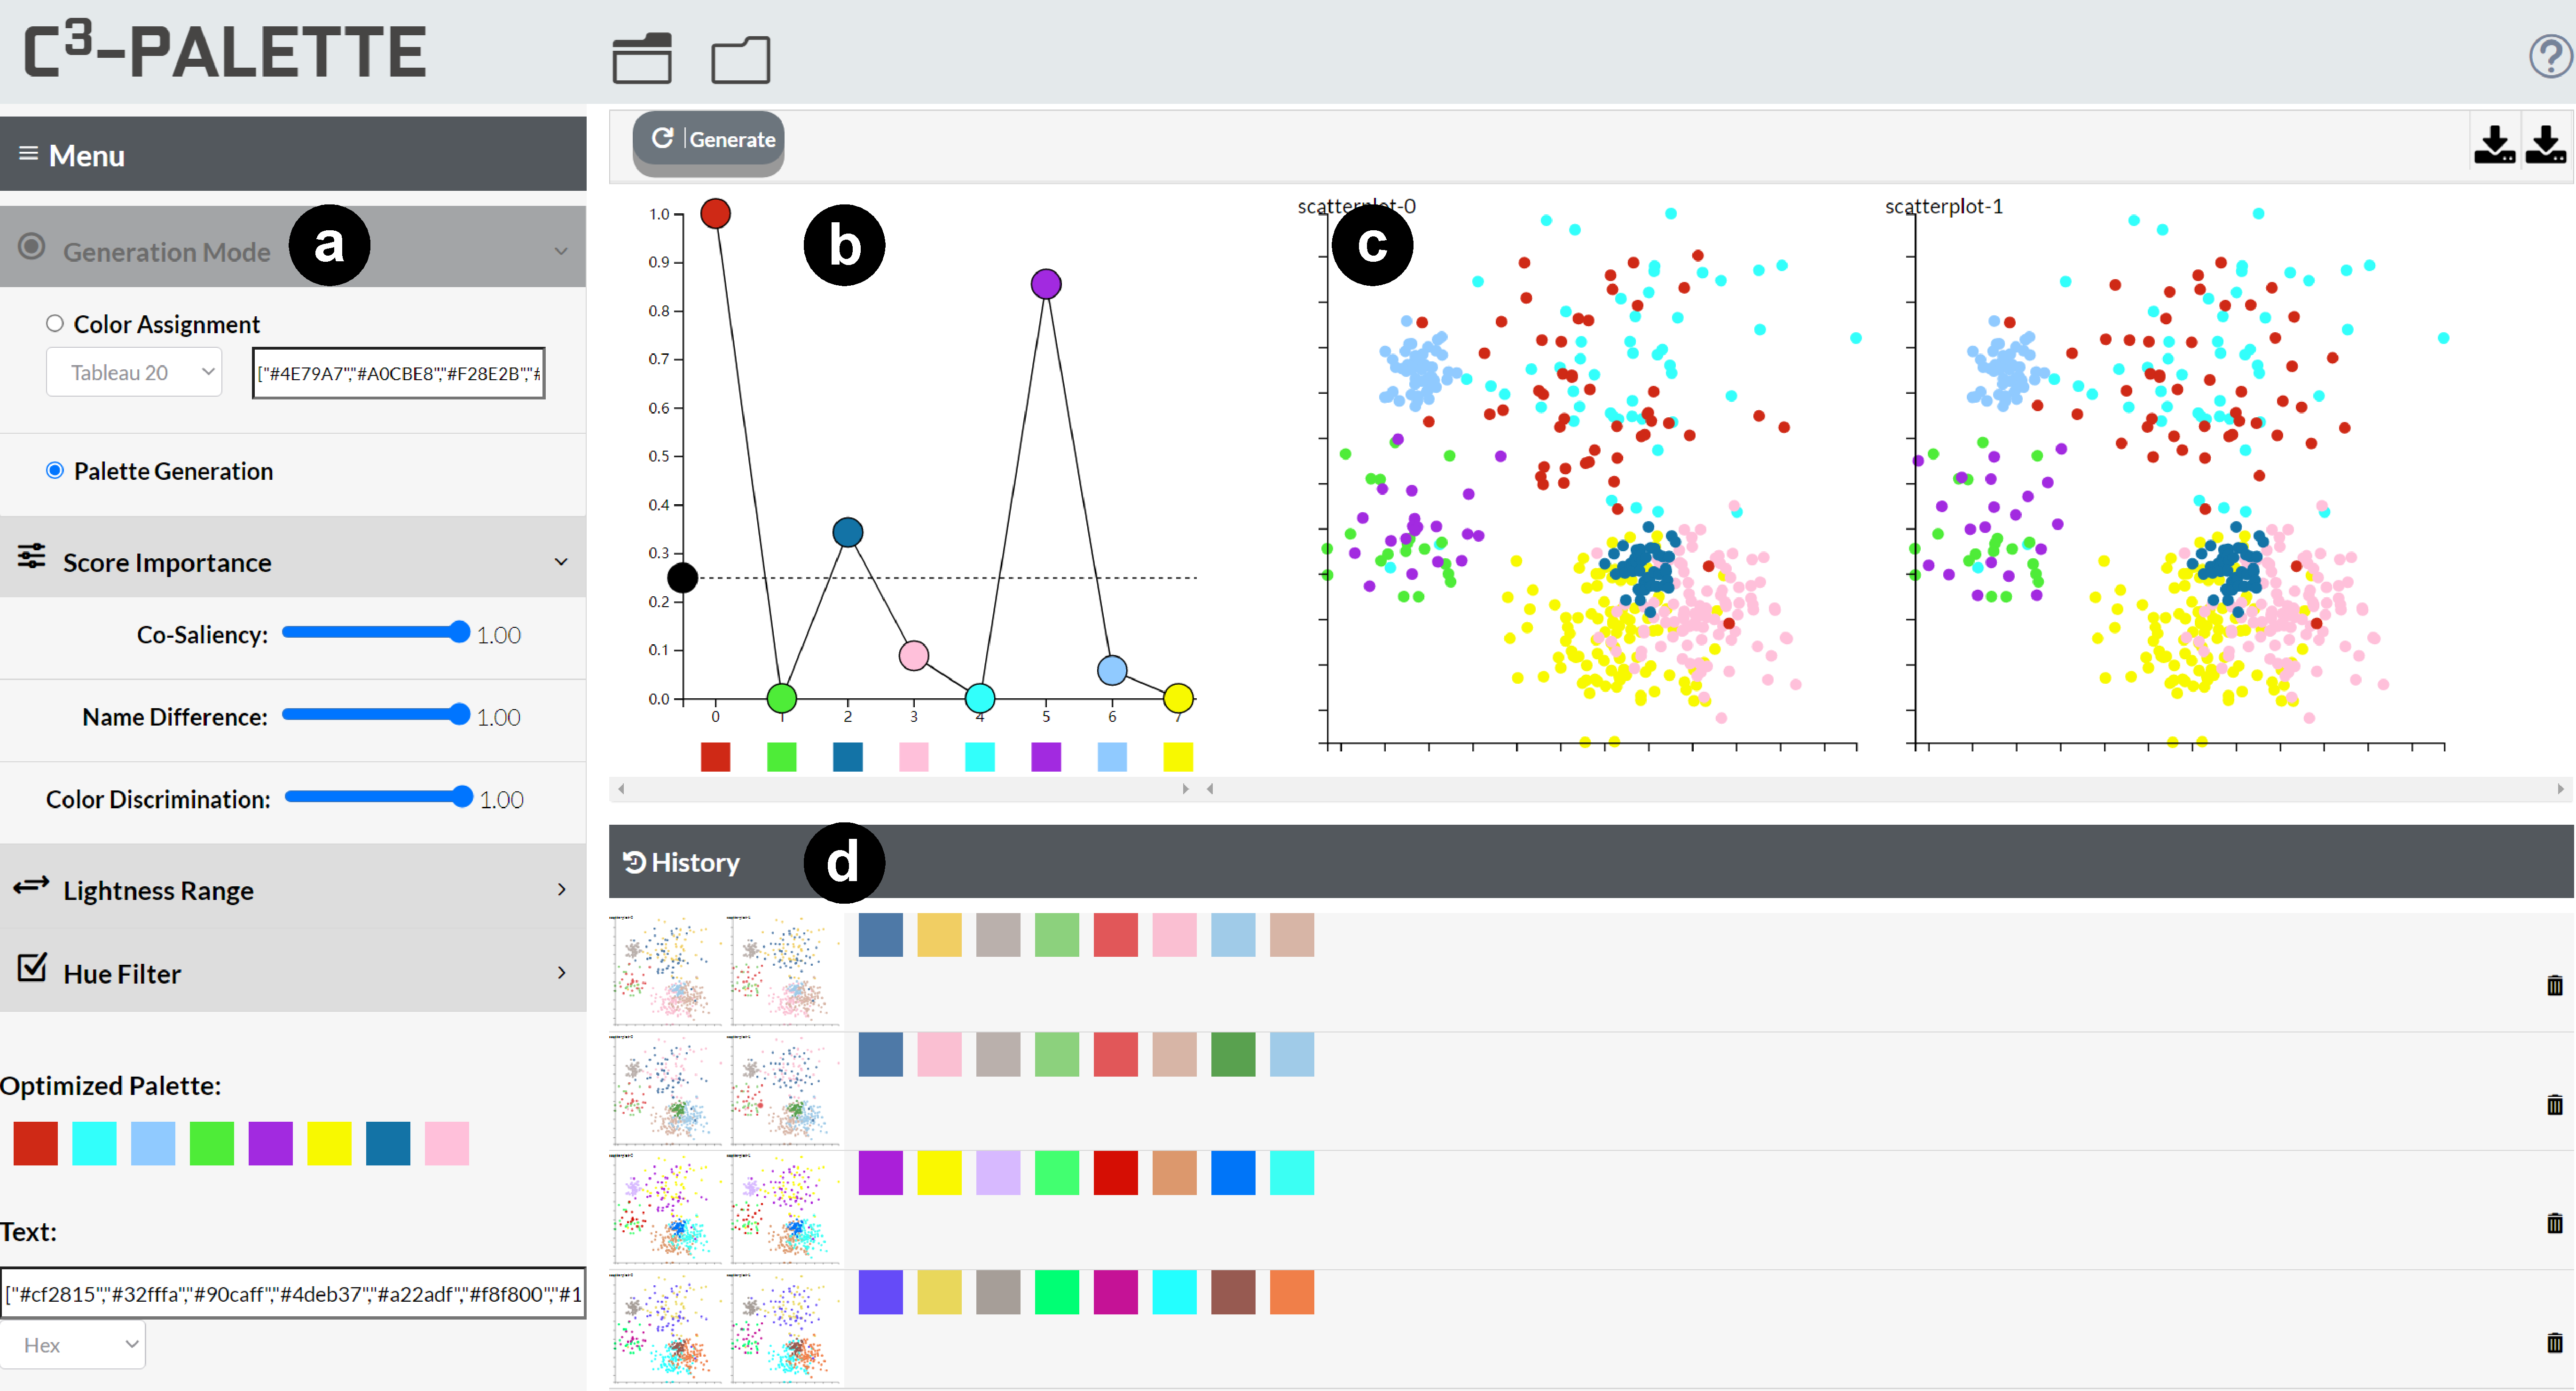
\includegraphics[width=1.0\columnwidth]{figures/interface.pdf}
\caption{Our interactive colorization system and a case study. (a) Screenshot of the interactive system consisted of four panels: (i) control panel; (ii) importance adjustment panel; (iii) visualization panel; and (iv) history panel. (b) Using this system to explore the changes of gases in an air quality data set~\cite{DEVITO2008750}: (top) The automatic generated palette creates salient colors for  lines; (middle, bottom) the palettes highlighting two lines with small changes generated by our methods without and with colour name constraint, respectively.}
\vspace*{-3mm}
\label{fig:ui-case}
\end{figure}

%\subsection{Interactive System}
\label{sec:interaction}
To help users interactively design colors for comparing multi-class scatterplots, we developed a web-based multi-view visualization tool \footnote{\small \url{https://c3-palette.github.io/}}
(see the screenshot in Fig.~\ref{fig:ui-case}(a)).
It consists of four coordinated views: (i) a control panel, (ii) an importance adjustment panel for adjusting $\kappa$ and  importance of each class, (iii) the juxtaposed visualizations, and (iv) a history view. 

After uploading multiple labeled datasets, the system automatically finds an optimal color mapping scheme to colorize the input data, while each class is encoded as a dot on the x-axis of the importance adjustment view indicating the change degree. If users like the color mapping scheme, they can save it to the history view. By default, our system finds a color mapping scheme to highlight the classes with large changes and renders the classes in ascending order of the corresponding change degrees. 
To facilitate a coherent exploration, we provide a color name constraint for  palette generation, where the consistency of color names will be preserved in the produced palettes.
If users like the color mapping scheme, they can save it to the history view.









\vspace{1.5mm}
\noindent\textbf{Color Name Constraints}.
Adjusting class importance and $\kappa$  allows to highlight some classes of interest with newly generated color palettes. However, this might not be intuitive for users, since the colors might be completely changed in the new palette. To address this issue,
one straightforward way is to  assign large  opacities  to classes of interest and small values to deemphasized classes, respectively. However, this method might not be able to pop out such classes, since their assigned colors are often have low contrast with the background (e.g., the yellow class in the top of Fig.~\ref{fig:ui-case}(b)).

To maintain consistent color schemes and highlight classes of interest, we introduce a color name constraint~\cite{heer2012color} for palette generation. Specifically, the name difference between the new color and the one in the previous palette should be smaller than a threshold during the search for new palettes.
In doing so, such selected classes can be easily identified from the new colorization results (see an example in the bottom of Fig.~\ref{fig:ui-case}(b)).




\subsection{Case Study}
\label{sec:caseStudy}


%\begin{figure}[!t]
%\centering
%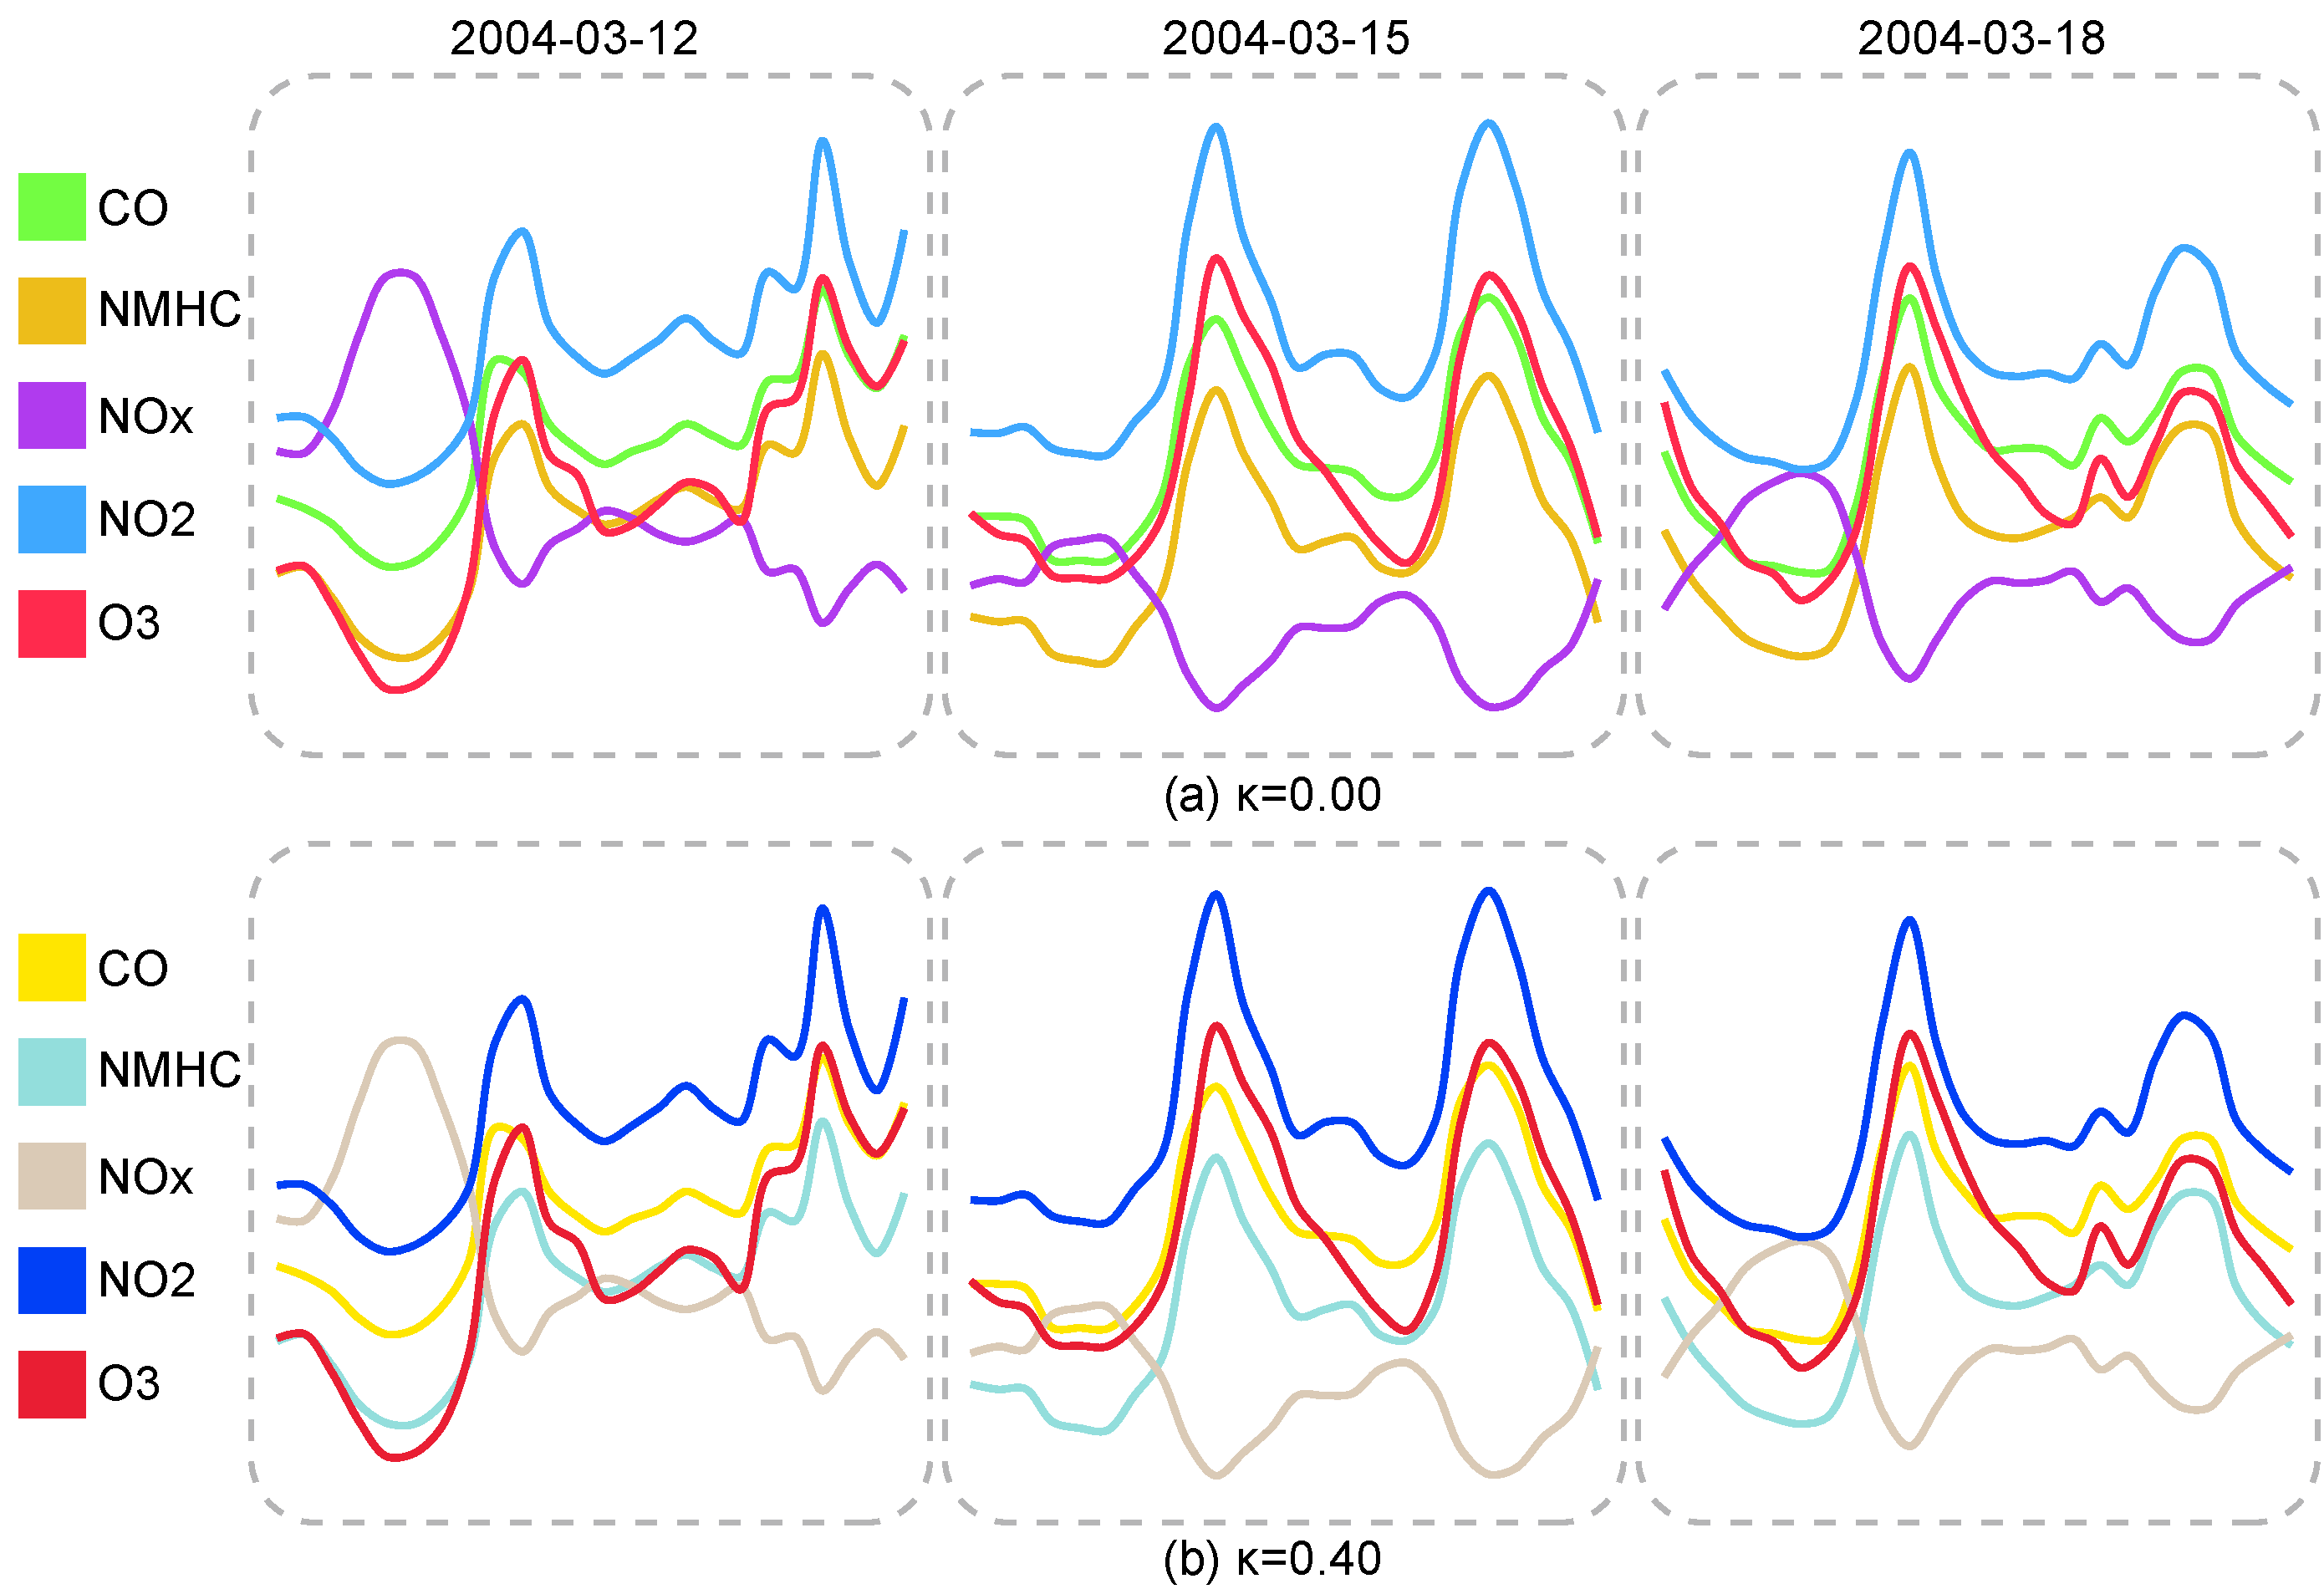
\includegraphics[width=0.96\linewidth]{figures/case-linechart.pdf}
%\caption{Exploring the changes of gases in an air quality data set~\cite{DEVITO2008750}. (a) The automatic generated palette creates salient colors for  all lines. (b) Two selected lines are popping out from the other lines in three views.}
%\vspace*{-3mm}
%\label{fig:caseStudy2}
%\end{figure}

To shed further light onto the ecological validity of our approach, we conducted a case study on a real-world categorical dataset visualized with line charts.
Here, we analyze an air quality data set ~\cite{DEVITO2008750} that contains hourly responses of a gas multi-sensor device deployed in an Italian city from March 12 to March 18, 2014.
The top in Fig.~\ref{fig:ui-case}(b) shows the juxtaposed line graphs encoded by our generated color palette, where each gas type is represented by a line with a unique color.
We can see that all gases are encoded with highly salient colors, making it hard to explore changes of specific gases. This is reasonable because the default $\kappa$ is zero, but all gases have large changes.
Thanks to our interaction mechanism, users can directly select classes of interest to be highlighted by assigning them with large importance, while  the $\theta$ values of the other classes are set to -1. Using the color name constrained palette generation method, the produced palette lets the selected lines pop out from the others (see the bottom in Fig.~\ref{fig:ui-case})). Hence, users can easily explore the changes of the selected two gases (NO$_2$ and O$_3$) in the three juxtaposed views.



\section {Conclusion and Future Work}
We presented $C^3$-palette, a data-aware approach for producing color
palettes for comparing horizontally juxtaposed categorical visualizations that allows a better identification of the biggest change between two data series, while maintaining the visual discrimination of classes. This goal is
achieved by a  novel co-saliency model, which characterizes the most co-salient features between juxtaposed labeled data visualizations while maintaining class discrimination in the individual visualizations. We evaluated $C^3$-palette through a crowd-sourcing study, which empirically demonstrates that our produced
palettes allow for an efficient visual comparison and good class discrimination.

Our work concentrated on juxtaposed comparisons to detect changes between multiple datasets, whereas its optimal color palette might not be appropriate for understanding other analytical comparison tasks (e.g., correlation tasks, rf.~\cite{Ondov19}. Future work needs to investigate the effectiveness and extensions of our approach for such comparison tasks. Furthermore, mark shape~\cite{liu2021data} and mark size~\cite{smart2019measuring}  might have an effect on the perceptual precision of visual comparisons and we will explore the possibility to model the influence of these factors. %In contrast, the number of marks only influences the efficiency for computing co-saliency, since our co-saliency is based on the nearest neighbourhood graphs built in the data space.

%Even the large datasets with multiple cases at the same position, our generated palettes still perform well.

Second, our approach produces colors with salient hue to highlight classes with large changes, but those colors do not visually indicate the ranking of class changes. It would be helpful to associate a color ordering constraint~\cite{Bujack18} with the degree of changes, so that the ranking of class changes can be shown clearly. On the other hand, our method can be extended to generate palettes for people with color vision deficiency by incorporating a physiologically-based model~\cite{machado2009physiologically} into our optimization framework.

Third, while our second user study only examined the interaction effect between change magnitude and different colorization methods, we plan to investigate how this effect is influenced by different types of changes in scatterplots, such as point number, center position and shape.
The order of rendering is critical for the comparison task and in this paper we treat it simply by rendering less important classes first. But when there are multiple important large classes at the same positions, less important classes might be overlapped and hard to distinguish. Thus a professional render order algorithm would be necessary for multi-class scatterplot rendering.

Last, our study only evaluated the effectiveness of our palettes with horizontally juxtaposed visualizations, while there are different layout methods such as vertical arrangement, mirrored arrangement, overlaid, and animation. Previous studies~\cite{Ondov19} show that animation performs well in identifying the largest difference and we will conduct studies to learn how well our palette works in this setting. On the other hand, there are a few 
different visual comparison methods~\cite{Gleicher11} such as plotting differences and faceting groups~\cite{wickham2009elegant}. It would be helpful to fully investigate the strengths and limitations of each of these methods for visual comparisons.




\section{Template Overview}
As noted in the introduction, the ``\verb|acmart|'' document class can
be used to prepare many different kinds of documentation --- a
double-blind initial submission of a full-length technical paper, a
two-page SIGGRAPH Emerging Technologies abstract, a ``camera-ready''
journal article, a SIGCHI Extended Abstract, and more --- all by
selecting the appropriate {\itshape template style} and {\itshape
  template parameters}.

This document will explain the major features of the document
class. For further information, the {\itshape \LaTeX\ User's Guide} is
available from
\url{https://www.acm.org/publications/proceedings-template}.

\subsection{Template Styles}

The primary parameter given to the ``\verb|acmart|'' document class is
the {\itshape template style} which corresponds to the kind of publication
or SIG publishing the work. This parameter is enclosed in square
brackets and is a part of the {\verb|documentclass|} command:
\begin{verbatim}
  \documentclass[STYLE]{acmart}
\end{verbatim}

Journals use one of three template styles. All but three ACM journals
use the {\verb|acmsmall|} template style:
\begin{itemize}
\item {\verb|acmsmall|}: The default journal template style.
\item {\verb|acmlarge|}: Used by JOCCH and TAP.
\item {\verb|acmtog|}: Used by TOG.
\end{itemize}

The majority of conference proceedings documentation will use the {\verb|acmconf|} template style.
\begin{itemize}
\item {\verb|acmconf|}: The default proceedings template style.
\item{\verb|sigchi|}: Used for SIGCHI conference articles.
\item{\verb|sigchi-a|}: Used for SIGCHI ``Extended Abstract'' articles.
\item{\verb|sigplan|}: Used for SIGPLAN conference articles.
\end{itemize}

\subsection{Template Parameters}

In addition to specifying the {\itshape template style} to be used in
formatting your work, there are a number of {\itshape template parameters}
which modify some part of the applied template style. A complete list
of these parameters can be found in the {\itshape \LaTeX\ User's Guide.}

Frequently-used parameters, or combinations of parameters, include:
\begin{itemize}
\item {\verb|anonymous,review|}: Suitable for a ``double-blind''
  conference submission. Anonymizes the work and includes line
  numbers. Use with the \verb|\acmSubmissionID| command to print the
  submission's unique ID on each page of the work.
\item{\verb|authorversion|}: Produces a version of the work suitable
  for posting by the author.
\item{\verb|screen|}: Produces colored hyperlinks.
\end{itemize}

This document uses the following string as the first command in the
source file:
\begin{verbatim}
\documentclass[sigconf,authordraft]{acmart}
\end{verbatim}

\section{Modifications}

Modifying the template --- including but not limited to: adjusting
margins, typeface sizes, line spacing, paragraph and list definitions,
and the use of the \verb|\vspace| command to manually adjust the
vertical spacing between elements of your work --- is not allowed.

{\bfseries Your document will be returned to you for revision if
  modifications are discovered.}

\section{Typefaces}

The ``\verb|acmart|'' document class requires the use of the
``Libertine'' typeface family. Your \TeX\ installation should include
this set of packages. Please do not substitute other typefaces. The
``\verb|lmodern|'' and ``\verb|ltimes|'' packages should not be used,
as they will override the built-in typeface families.

\section{Title Information}

The title of your work should use capital letters appropriately -
\url{https://capitalizemytitle.com/} has useful rules for
capitalization. Use the {\verb|title|} command to define the title of
your work. If your work has a subtitle, define it with the
{\verb|subtitle|} command.  Do not insert line breaks in your title.

If your title is lengthy, you must define a short version to be used
in the page headers, to prevent overlapping text. The \verb|title|
command has a ``short title'' parameter:
\begin{verbatim}
  \title[short title]{full title}
\end{verbatim}

\section{Authors and Affiliations}

Each author must be defined separately for accurate metadata
identification. Multiple authors may share one affiliation. Authors'
names should not be abbreviated; use full first names wherever
possible. Include authors' e-mail addresses whenever possible.

Grouping authors' names or e-mail addresses, or providing an ``e-mail
alias,'' as shown below, is not acceptable:
\begin{verbatim}
  \author{Brooke Aster, David Mehldau}
  \email{dave,judy,steve@university.edu}
  \email{firstname.lastname@phillips.org}
\end{verbatim}

The \verb|authornote| and \verb|authornotemark| commands allow a note
to apply to multiple authors --- for example, if the first two authors
of an article contributed equally to the work.

If your author list is lengthy, you must define a shortened version of
the list of authors to be used in the page headers, to prevent
overlapping text. The following command should be placed just after
the last \verb|\author{}| definition:
\begin{verbatim}
  \renewcommand{\shortauthors}{McCartney, et al.}
\end{verbatim}
Omitting this command will force the use of a concatenated list of all
of the authors' names, which may result in overlapping text in the
page headers.

The article template's documentation, available at
\url{https://www.acm.org/publications/proceedings-template}, has a
complete explanation of these commands and tips for their effective
use.

Note that authors' addresses are mandatory for journal articles.

\section{Rights Information}

Authors of any work published by ACM will need to complete a rights
form. Depending on the kind of work, and the rights management choice
made by the author, this may be copyright transfer, permission,
license, or an OA (open access) agreement.

Regardless of the rights management choice, the author will receive a
copy of the completed rights form once it has been submitted. This
form contains \LaTeX\ commands that must be copied into the source
document. When the document source is compiled, these commands and
their parameters add formatted text to several areas of the final
document:
\begin{itemize}
\item the ``ACM Reference Format'' text on the first page.
\item the ``rights management'' text on the first page.
\item the conference information in the page header(s).
\end{itemize}

Rights information is unique to the work; if you are preparing several
works for an event, make sure to use the correct set of commands with
each of the works.

The ACM Reference Format text is required for all articles over one
page in length, and is optional for one-page articles (abstracts).

\section{CCS Concepts and User-Defined Keywords}

Two elements of the ``acmart'' document class provide powerful
taxonomic tools for you to help readers find your work in an online
search.

The ACM Computing Classification System ---
\url{https://www.acm.org/publications/class-2012} --- is a set of
classifiers and concepts that describe the computing
discipline. Authors can select entries from this classification
system, via \url{https://dl.acm.org/ccs/ccs.cfm}, and generate the
commands to be included in the \LaTeX\ source.

User-defined keywords are a comma-separated list of words and phrases
of the authors' choosing, providing a more flexible way of describing
the research being presented.

CCS concepts and user-defined keywords are required for for all
articles over two pages in length, and are optional for one- and
two-page articles (or abstracts).

\section{Sectioning Commands}

Your work should use standard \LaTeX\ sectioning commands:
\verb|section|, \verb|subsection|, \verb|subsubsection|, and
\verb|paragraph|. They should be numbered; do not remove the numbering
from the commands.

Simulating a sectioning command by setting the first word or words of
a paragraph in boldface or italicized text is {\bfseries not allowed.}

\section{Tables}

The ``\verb|acmart|'' document class includes the ``\verb|booktabs|''
package --- \url{https://ctan.org/pkg/booktabs} --- for preparing
high-quality tables.

Table captions are placed {\itshape above} the table.

Because tables cannot be split across pages, the best placement for
them is typically the top of the page nearest their initial cite.  To
ensure this proper ``floating'' placement of tables, use the
environment \textbf{table} to enclose the table's contents and the
table caption.  The contents of the table itself must go in the
\textbf{tabular} environment, to be aligned properly in rows and
columns, with the desired horizontal and vertical rules.  Again,
detailed instructions on \textbf{tabular} material are found in the
\textit{\LaTeX\ User's Guide}.

Immediately following this sentence is the point at which
Table~\ref{tab:freq} is included in the input file; compare the
placement of the table here with the table in the printed output of
this document.

\begin{table}
  \caption{Frequency of Special Characters}
  \label{tab:freq}
  \begin{tabular}{ccl}
    \toprule
    Non-English or Math&Frequency&Comments\\
    \midrule
    \O & 1 in 1,000& For Swedish names\\
    $\pi$ & 1 in 5& Common in math\\
    \$ & 4 in 5 & Used in business\\
    $\Psi^2_1$ & 1 in 40,000& Unexplained usage\\
  \bottomrule
\end{tabular}
\end{table}

To set a wider table, which takes up the whole width of the page's
live area, use the environment \textbf{table*} to enclose the table's
contents and the table caption.  As with a single-column table, this
wide table will ``float'' to a location deemed more
desirable. Immediately following this sentence is the point at which
Table~\ref{tab:commands} is included in the input file; again, it is
instructive to compare the placement of the table here with the table
in the printed output of this document.

\begin{table*}
  \caption{Some Typical Commands}
  \label{tab:commands}
  \begin{tabular}{ccl}
    \toprule
    Command &A Number & Comments\\
    \midrule
    \texttt{{\char'134}author} & 100& Author \\
    \texttt{{\char'134}table}& 300 & For tables\\
    \texttt{{\char'134}table*}& 400& For wider tables\\
    \bottomrule
  \end{tabular}
\end{table*}

Always use midrule to separate table header rows from data rows, and
use it only for this purpose. This enables assistive technologies to
recognise table headers and support their users in navigating tables
more easily.

\section{Math Equations}
You may want to display math equations in three distinct styles:
inline, numbered or non-numbered display.  Each of the three are
discussed in the next sections.

\subsection{Inline (In-text) Equations}
A formula that appears in the running text is called an inline or
in-text formula.  It is produced by the \textbf{math} environment,
which can be invoked with the usual
\texttt{{\char'134}begin\,\ldots{\char'134}end} construction or with
the short form \texttt{\$\,\ldots\$}. You can use any of the symbols
and structures, from $\alpha$ to $\omega$, available in
\LaTeX~\cite{Lamport:LaTeX}; this section will simply show a few
examples of in-text equations in context. Notice how this equation:
\begin{math}
  \lim_{n\rightarrow \infty}x=0
\end{math},
set here in in-line math style, looks slightly different when
set in display style.  (See next section).

\subsection{Display Equations}
A numbered display equation---one set off by vertical space from the
text and centered horizontally---is produced by the \textbf{equation}
environment. An unnumbered display equation is produced by the
\textbf{displaymath} environment.

Again, in either environment, you can use any of the symbols and
structures available in \LaTeX\@; this section will just give a couple
of examples of display equations in context.  First, consider the
equation, shown as an inline equation above:
\begin{equation}
  \lim_{n\rightarrow \infty}x=0
\end{equation}
Notice how it is formatted somewhat differently in
the \textbf{displaymath}
environment.  Now, we'll enter an unnumbered equation:
\begin{displaymath}
  \sum_{i=0}^{\infty} x + 1
\end{displaymath}
and follow it with another numbered equation:
\begin{equation}
  \sum_{i=0}^{\infty}x_i=\int_{0}^{\pi+2} f
\end{equation}
just to demonstrate \LaTeX's able handling of numbering.

\section{Figures}

The ``\verb|figure|'' environment should be used for figures. One or
more images can be placed within a figure. If your figure contains
third-party material, you must clearly identify it as such, as shown
in the example below.
%\begin{figure}[h]
%  \centering
%  \includegraphics[width=\linewidth]{}
%  \caption{1907 Franklin Model D roadster. Photograph by Harris \&
%    Ewing, Inc. [Public domain], via Wikimedia
%    Commons. (\url{https://goo.gl/VLCRBB}).}
%  \Description{A woman and a girl in white dresses sit in an open car.}
%\end{figure}

Your figures should contain a caption which describes the figure to
the reader.

Figure captions are placed {\itshape below} the figure.

Every figure should also have a figure description unless it is purely
decorative. These descriptions convey what’s in the image to someone
who cannot see it. They are also used by search engine crawlers for
indexing images, and when images cannot be loaded.

A figure description must be unformatted plain text less than 2000
characters long (including spaces).  {\bfseries Figure descriptions
  should not repeat the figure caption – their purpose is to capture
  important information that is not already provided in the caption or
  the main text of the paper.} For figures that convey important and
complex new information, a short text description may not be
adequate. More complex alternative descriptions can be placed in an
appendix and referenced in a short figure description. For example,
provide a data table capturing the information in a bar chart, or a
structured list representing a graph.  For additional information
regarding how best to write figure descriptions and why doing this is
so important, please see
\url{https://www.acm.org/publications/taps/describing-figures/}.

\subsection{The ``Teaser Figure''}

A ``teaser figure'' is an image, or set of images in one figure, that
are placed after all author and affiliation information, and before
the body of the article, spanning the page. If you wish to have such a
figure in your article, place the command immediately before the
\verb|\maketitle| command:
\begin{verbatim}
  \begin{teaserfigure}
    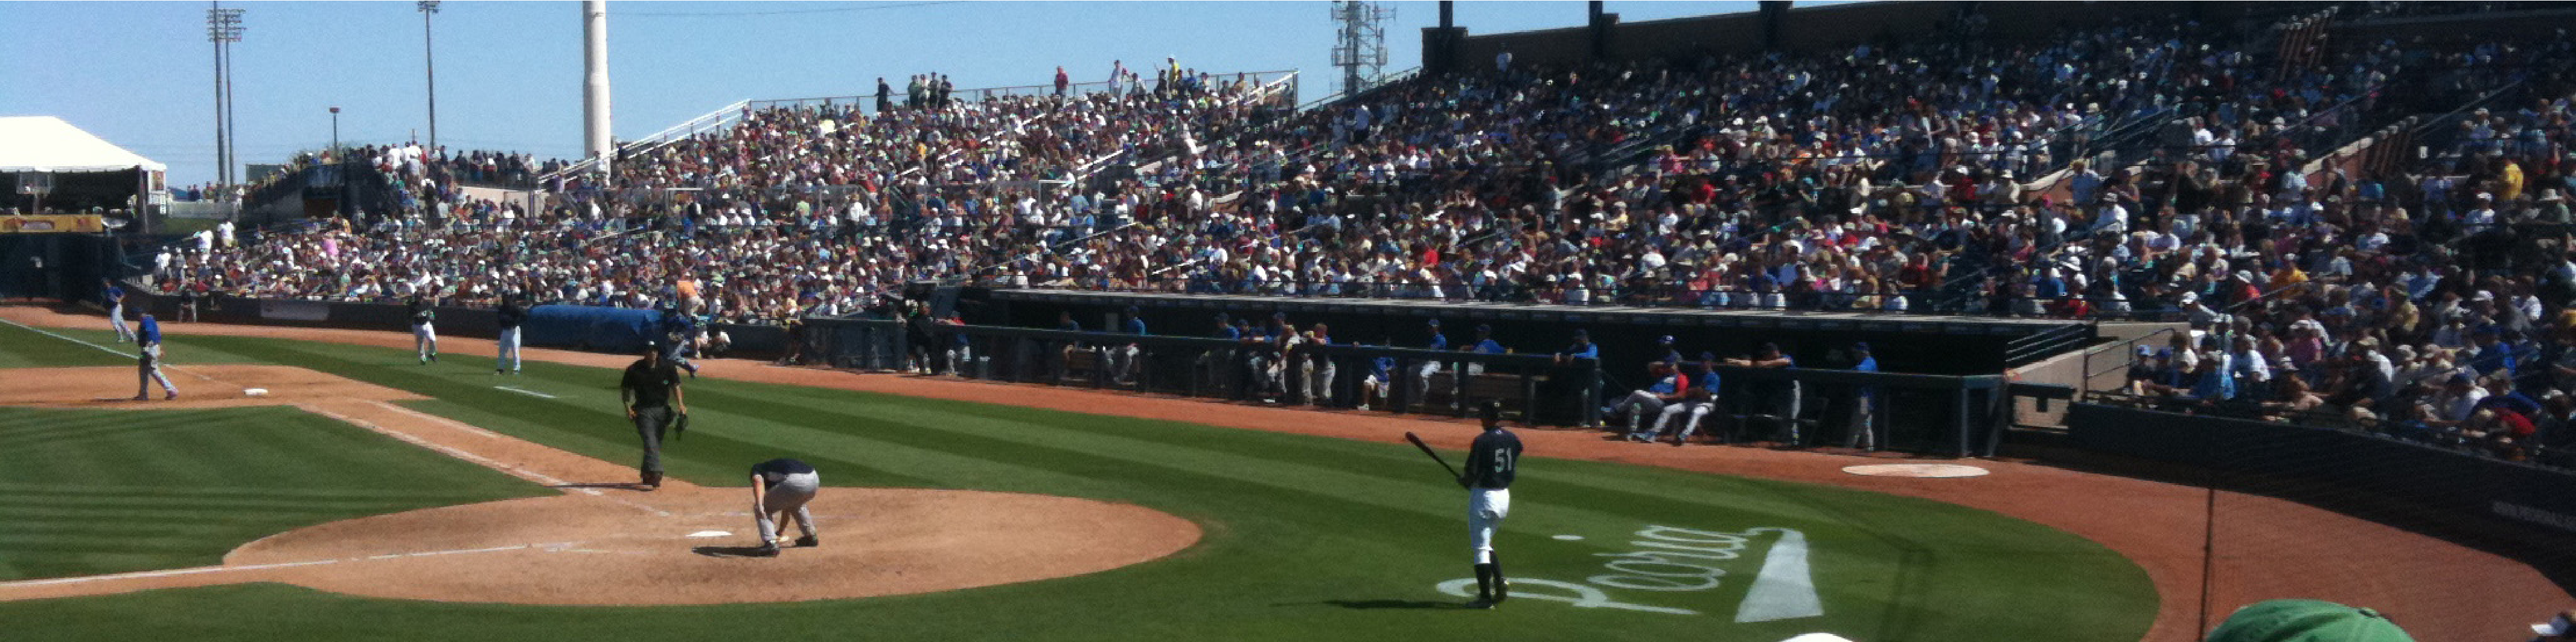
\includegraphics[width=\textwidth]{sampleteaser}
    \caption{figure caption}
    \Description{figure description}
  \end{teaserfigure}
\end{verbatim}

\section{Citations and Bibliographies}

The use of \BibTeX\ for the preparation and formatting of one's
references is strongly recommended. Authors' names should be complete
--- use full first names (``Donald E. Knuth'') not initials
(``D. E. Knuth'') --- and the salient identifying features of a
reference should be included: title, year, volume, number, pages,
article DOI, etc.

The bibliography is included in your source document with these two
commands, placed just before the \verb|\end{document}| command:
\begin{verbatim}
  \bibliographystyle{ACM-Reference-Format}
  \bibliography{bibfile}
\end{verbatim}
where ``\verb|bibfile|'' is the name, without the ``\verb|.bib|''
suffix, of the \BibTeX\ file.

Citations and references are numbered by default. A small number of
ACM publications have citations and references formatted in the
``author year'' style; for these exceptions, please include this
command in the {\bfseries preamble} (before the command
``\verb|\begin{document}|'') of your \LaTeX\ source:
\begin{verbatim}
  \citestyle{acmauthoryear}
\end{verbatim}

  Some examples.  A paginated journal article \cite{Abril07}, an
  enumerated journal article \cite{Cohen07}, a reference to an entire
  issue \cite{JCohen96}, a monograph (whole book) \cite{Kosiur01}, a
  monograph/whole book in a series (see 2a in spec. document)
  \cite{Harel79}, a divisible-book such as an anthology or compilation
  \cite{Editor00} followed by the same example, however we only output
  the series if the volume number is given \cite{Editor00a} (so
  Editor00a's series should NOT be present since it has no vol. no.),
  a chapter in a divisible book \cite{Spector90}, a chapter in a
  divisible book in a series \cite{Douglass98}, a multi-volume work as
  book \cite{Knuth97}, a couple of articles in a proceedings (of a
  conference, symposium, workshop for example) (paginated proceedings
  article) \cite{Andler79, Hagerup1993}, a proceedings article with
  all possible elements \cite{Smith10}, an example of an enumerated
  proceedings article \cite{VanGundy07}, an informally published work
  \cite{Harel78}, a couple of preprints \cite{Bornmann2019,
    AnzarootPBM14}, a doctoral dissertation \cite{Clarkson85}, a
  master's thesis: \cite{anisi03}, an online document / world wide web
  resource \cite{Thornburg01, Ablamowicz07, Poker06}, a video game
  (Case 1) \cite{Obama08} and (Case 2) \cite{Novak03} and \cite{Lee05}
  and (Case 3) a patent \cite{JoeScientist001}, work accepted for
  publication \cite{rous08}, 'YYYYb'-test for prolific author
  \cite{SaeediMEJ10} and \cite{SaeediJETC10}. Other cites might
  contain 'duplicate' DOI and URLs (some SIAM articles)
  \cite{Kirschmer:2010:AEI:1958016.1958018}. Boris / Barbara Beeton:
  multi-volume works as books \cite{MR781536} and \cite{MR781537}. A
  couple of citations with DOIs:
  \cite{2004:ITE:1009386.1010128,Kirschmer:2010:AEI:1958016.1958018}. Online
  citations: \cite{TUGInstmem, Thornburg01, CTANacmart}. Artifacts:
  \cite{R} and \cite{UMassCitations}.

\section{Acknowledgments}

Identification of funding sources and other support, and thanks to
individuals and groups that assisted in the research and the
preparation of the work should be included in an acknowledgment
section, which is placed just before the reference section in your
document.

This section has a special environment:
\begin{verbatim}
  \begin{acks}
  ...
  \end{acks}
\end{verbatim}
so that the information contained therein can be more easily collected
during the article metadata extraction phase, and to ensure
consistency in the spelling of the section heading.

Authors should not prepare this section as a numbered or unnumbered {\verb|\section|}; please use the ``{\verb|acks|}'' environment.

\section{Appendices}

If your work needs an appendix, add it before the
``\verb|\end{document}|'' command at the conclusion of your source
document.

Start the appendix with the ``\verb|appendix|'' command:
\begin{verbatim}
  \appendix
\end{verbatim}
and note that in the appendix, sections are lettered, not
numbered. This document has two appendices, demonstrating the section
and subsection identification method.

\section{SIGCHI Extended Abstracts}

The ``\verb|sigchi-a|'' template style (available only in \LaTeX\ and
not in Word) produces a landscape-orientation formatted article, with
a wide left margin. Three environments are available for use with the
``\verb|sigchi-a|'' template style, and produce formatted output in
the margin:
\begin{itemize}
\item {\verb|sidebar|}:  Place formatted text in the margin.
\item {\verb|marginfigure|}: Place a figure in the margin.
\item {\verb|margintable|}: Place a table in the margin.
\end{itemize}

%%
%% The acknowledgments section is defined using the "acks" environment
%% (and NOT an unnumbered section). This ensures the proper
%% identification of the section in the article metadata, and the
%% consistent spelling of the heading.
\begin{acks}
To Robert, for the bagels and explaining CMYK and color spaces.
\end{acks}

%%
%% The next two lines define the bibliography style to be used, and
%% the bibliography file.
\bibliographystyle{ACM-Reference-Format}
\bibliography{coSaliency}

%%
%% If your work has an appendix, this is the place to put it.
\appendix

\section{Research Methods}

\subsection{Part One}

Lorem ipsum dolor sit amet, consectetur adipiscing elit. Morbi
malesuada, quam in pulvinar varius, metus nunc fermentum urna, id
sollicitudin purus odio sit amet enim. Aliquam ullamcorper eu ipsum
vel mollis. Curabitur quis dictum nisl. Phasellus vel semper risus, et
lacinia dolor. Integer ultricies commodo sem nec semper.

\subsection{Part Two}

Etiam commodo feugiat nisl pulvinar pellentesque. Etiam auctor sodales
ligula, non varius nibh pulvinar semper. Suspendisse nec lectus non
ipsum convallis congue hendrerit vitae sapien. Donec at laoreet
eros. Vivamus non purus placerat, scelerisque diam eu, cursus
ante. Etiam aliquam tortor auctor efficitur mattis.

\section{Online Resources}

Nam id fermentum dui. Suspendisse sagittis tortor a nulla mollis, in
pulvinar ex pretium. Sed interdum orci quis metus euismod, et sagittis
enim maximus. Vestibulum gravida massa ut felis suscipit
congue. Quisque mattis elit a risus ultrices commodo venenatis eget
dui. Etiam sagittis eleifend elementum.

Nam interdum magna at lectus dignissim, ac dignissim lorem
rhoncus. Maecenas eu arcu ac neque placerat aliquam. Nunc pulvinar
massa et mattis lacinia.

\end{document}
\endinput
%%
%% End of file `sample-authordraft.tex'.
